
\documentclass[10pt,letterpaper]{article}

\usepackage[preprint]{arxiv}

\widowpenalty10000
\clubpenalty10000
\setlength{\textfloatsep}{1pt}
\setlength{\abovecaptionskip}{2pt} 
\setlength{\belowcaptionskip}{2pt} 


\setlength{\abovedisplayskip}{1pt}
\setlength{\belowdisplayskip}{1pt}
\setlength{\abovedisplayshortskip}{1pt}
\setlength{\belowdisplayshortskip}{1pt}

\setcitestyle{square, comma, numbers,sort&compress, super}
\usepackage{enumitem}
\usepackage{algpseudocode}
\usepackage[font=small,labelfont=bf]{caption}
\usepackage{array}
\usepackage{multirow}
\usepackage{booktabs}
\usepackage{algorithm}
\usepackage{subcaption}
\usepackage[normalem]{ulem}
\usepackage{xparse}
\usepackage{pifont}
\usepackage{bm}
\usepackage{threeparttable}
\usepackage{etoolbox}

\usepackage{listings}
\usepackage{mwe} %
\usepackage{makecell}
\usepackage{color, colortbl}
\usepackage{tabularx}
\usepackage{pifont}%
\usepackage[accsupp]{axessibility}
\usepackage[symbol]{footmisc}
\usepackage{pgfplots}
\usetikzlibrary{spy}
\usepackage[scaled=0.85]{DejaVuSansMono}
\usepackage{minitoc}

%
% --- inline annotations
%
\newcommand{\red}[1]{{\color{red}#1}}
\newcommand{\todo}[1]{{\color{red}#1}}
\newcommand{\TODO}[1]{\textbf{\color{red}[TODO: #1]}}
% --- disable by uncommenting  
% \renewcommand{\TODO}[1]{}
% \renewcommand{\todo}[1]{#1}



\definecolor{citecolor}{HTML}{0071bc}


\crefname{section}{\S}{\S\S}


\def\paperID{3287} %
\def\confName{ICCV}
\def\confYear{2025}

\title{Scaling Laws for Native Multimodal Models}



\author{
    Mustafa Shukor\thanks{Work done during an internship at Apple.} \\
    Sorbonne University
    \And
    Enrico Fini \\
    Apple
    \And
    Victor Guilherme Turrisi da Costa \\
    Apple
    \And
    Matthieu Cord \\
    Sorbonne University 
    \And
    Joshua Susskind \\
    Apple
    \And
    Alaaeldin El-Nouby \\
    Apple   
}

\renewcommand \thepart{}
\renewcommand \partname{}

\begin{document}
\setcounter{tocdepth}{2}
\doparttoc %
\renewcommand\ptctitle{}
\faketableofcontents %

\maketitle

\begin{abstract}
Fine-tuning provides an effective means to specialize pre-trained models for various downstream tasks. However, fine-tuning often incurs high memory overhead, especially for large transformer-based models, such as LLMs. While existing methods may reduce certain parts of the memory required for fine-tuning, they still require caching all intermediate activations computed in the forward pass to update weights during the backward pass. In~this work, we develop \method, a method to reduce memory usage,  specifically the memory to store intermediate activations, in the fine-tuning of transformer-based models. During the backward pass, \method approximates the gradient computation by backpropagating through just a subset of input tokens. Thus, with \method, only a subset of intermediate activations are cached during the forward pass. Also, \method can be easily combined with existing methods like LoRA, further reducing the memory cost. We evaluate our approach on pre-trained transformer models with up to billions of parameters, considering the performance on multiple downstream tasks such as text classification and question answering in a few-shot learning setup. Overall, \method achieves performance on par with full fine-tuning or representative memory-efficient fine-tuning methods,  while greatly reducing the memory footprint, especially when combined with other methods with complementary memory reduction mechanisms. We hope that our approach will facilitate the fine-tuning of large transformers,  in specializing them for specific domains or co-training them with other neural components from a larger system. Our code is available at \githubURL.
\blfootnote{\textbf{*} Equal contribution}
\end{abstract}
    
\section{Introduction}
\label{sec:intro}

\begin{figure*}[t!]
    \centering
    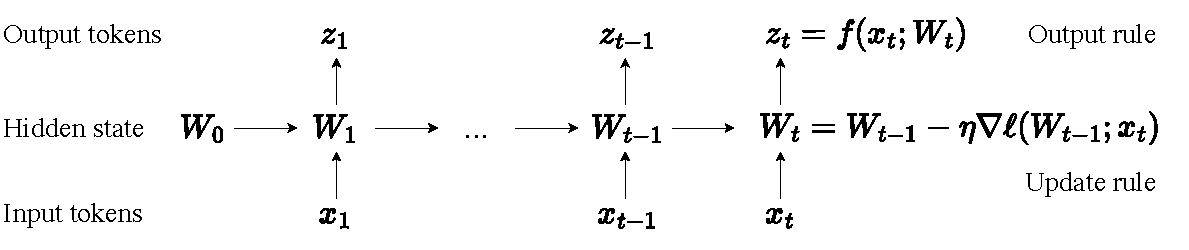
\includegraphics[width=0.8\textwidth]{figs/simple_teaser.pdf}
    \caption{All RNN layers can be expressed as a hidden state that transitions according to an update rule.
    The key idea in \cite{sun2024ttt} is to make the hidden state itself a model $f$ with weights $W$, and the update rule a gradient step on the self-supervised loss $\ell$.
    Therefore, updating the hidden state on a test sequence is equivalent to training the model $f$ at test time. 
    This process, known as Test-Time Training (TTT), is programmed into TTT layers. 
    Figure and caption taken from \cite{sun2024ttt}.
    }
    \label{fig:ttt-layer}
\end{figure*}

Despite the remarkable progress in visual and physical realism, state-of-the-art video Transformers are still generating mostly short clips of single scenes without complex stories.
At the time of writing (March 2025), the maximum length of public APIs for video generation is 20 seconds for Sora (OpenAI), 16 seconds for MovieGen (Meta), 10 for Ray~2 (Luma), and 8 for Veo~2 (Google).
None of these APIs can autonomously generate complex multi-scene stories.

A fundamental challenge behind these technical limitations is long context, because the cost of self-attention layers in Transformers increases quadratically with context length.
This challenge is especially acute for video generation with dynamic motion, whose context cannot be easily compressed by a tokenizer.
Using a standard tokenizer, each of our one-minute videos requires over 300k tokens in context. 
With self-attention, generating a one-minute video would have taken $11\times$ longer than generating 20 videos of 3 seconds each, and training would have taken $12\times$ longer.

To address this challenge, recent work on video generation has investigated RNN layers as an efficient alternative to self-attention, because their cost increases linearly with context length~\cite{wang2024lingenhighresolutionminutelengthtexttovideo}.
Modern RNN layers, especially variants of linear attention~\cite{schmidhuberlinearattn, katharopoulos2020lineartransformers} such as Mamba~\cite{gu2024mamba, dao2024mamba2} and DeltaNet~\cite{schlag2021deltanet, yang2025gateddeltanetworksimproving}, have shown impressive results for natural language tasks.
However, we have yet to see long videos with complex stories or dynamic motion generated by RNNs.
Videos (\href{https://lineargen.github.io/}{link}) in \cite{wang2024lingenhighresolutionminutelengthtexttovideo} are high resolution and one-minute long, but contain only single scenes and slow motion, let alone complex stories.

We believe that these RNN layers generate less complex videos because their hidden states are less expressive.
RNN layers can only store past tokens into a hidden state of fixed size, which is only a matrix for linear attention variants such as Mamba and DeltaNet.
It is inherently challenging to compress hundreds of thousands of vectors into a matrix with only thousands in rank.
As a consequence, these RNN layers struggle to remember the deep relationships between distant tokens.

We experiment with an alternative class of RNN layers whose hidden states themselves can be neural networks. Specifically, we use two-layer MLPs with 2$\times$ more hidden cells and richer nonlinearities than the linear (matrix) hidden states in linear attention variants.
Since the neural network hidden states are updated by training even on test sequences, these new layers are called Test-Time Training (TTT) layers~\cite{sun2024ttt}.

We start from a pre-trained Diffusion Transformer (CogVideo-X 5B \cite{hong2023cogvideo}) that could only generate 3-second short clips at 16 fps (or 6 seconds at 8 fps).
Then, we add TTT layers initialized from scratch and fine-tune this model to generate one-minute videos from text storyboards. 
We limit the self-attention layers to 3-second segments so their cost stays manageable.
With only preliminary systems optimization, our training run takes the equivalent of 50 hours on 256 H100s.

We curate a text-to-video dataset based on $\approx$ 7 hours of \textit{Tom and Jerry} cartoons with human-annotated storyboards.
We intentionally limit our scope to this specific domain for fast research iteration.
As a proof-of-concept, our dataset emphasizes complex, multi-scene, and long-range stories with dynamic motion, where progress is still needed; it has less emphasis on visual and physical realism, where remarkable progress has already been made.
We believe that improvements in long-context capabilities for this specific domain will transfer to general-purpose video generation.

Compared to strong baselines such as Mamba 2~\cite{dao2024mamba2}, Gated DeltaNet~\cite{yang2025gateddeltanetworksimproving}, and sliding-window attention layers, TTT layers generate much more coherent videos that tell complex stories with dynamic motion, leading by 34 Elo points in a human evaluation of 100 videos per method.
For context, GPT-4o scores 29 Elo points over GPT-4 Turbo in LMSys Chatbot Arena~\cite{chiang2024chatbot}.

Sample videos, code and annotations are available at:
\url{https://test-time-training.github.io/video-dit}
\section{Preliminaries}



\subsection{Definitions}

\cpar{Native Multimodal Models (NMMs):}
Models that are trained from scratch on all modalities simultaneously without
relying on pre-trained LLMs or vision encoders. Our focus is on the
representative image and text modalities, where the model processes both text
and images as input and generates text as output.

\cpar{Early fusion:} Enabling multimodal interaction from the beginning, using
almost no modality-specific parameters (\eg, except a linear layer to patchify
images). Using a single transformer model, this approach processes raw
multimodal \edit{input—tokenized text and continuous image patches—with no
image discretization.} \edit{We} refer to the main transformer as
the decoder.

\cpar{Late fusion:} Delaying the multimodal interaction \edit{to} deeper layers,
typically after separate unimodal components \edit{has processed} each modality
independently (\eg, a vision encoder connected to an LLM).

\cpar{Modality-agnostic routing:} In sparse mixture-of-experts, \edit{modality-agnostic} routing
refers to relying on a learned router module that is trained jointly with the
model.

\cpar{Modality-aware routing:} Routing based on pre-defined rules such as
routing based on the modality type (\eg, vision-tokens, token-tokens).

\begin{table}[t!]
    \centering
    \setlength{\tabcolsep}{8pt}
    \renewcommand{\arraystretch}{1.0}
    \resizebox{1\linewidth}{!}{
    \begin{tabular}{c p{0.999\linewidth}}
         Expression & Definition  \\
         \shline
         \textbf{$N$}     & \normalfont{{Number of parameters in the multimodal decoder. For MoEs this refers to the \edit{active parameters.}}} \\
         \grayrow
         \textbf{$D$}     & \normalfont{{Total number of multimodal tokens.}} \\
         \textbf{$N_{v}$} & \normalfont{{Number of vision-only tokens.}} \\
         \grayrow
         \textbf{$D_{v}$} & \normalfont{{Number of parameters in the vision-specific encoder. Only exists in late-fusion architectures.}} \\
         \textbf{$C$}     & \small{{Total number of FLOPs, estimated as $C=6ND$ for early-fusion and $C=6(N_vD_v+ND)$ for late-fusion.}} \\
         \grayrow
         \textbf{$L$}     & \normalfont{{Average validation loss on interleaved image-text, image-caption, and text-only data mixtures.}} \\
    \end{tabular}}
    \caption{Definitions of the expressions used throughout the paper.}
    \label{tab:my_label}
\end{table}




\subsection{Scaling Laws}
We aim to understand the scaling properties of NMMs and how different
architectural choices influence trade-offs. To this end, we analyze our models
within the scaling laws framework proposed by~\citet{kaplan2020scaling,
hoffmann2022training}.
We compute FLOPs based on the total number of parameters, using the
approximation \(C = 6ND\), as adopted in prior
work~\citep{hoffmann2022training,abnar2025parameters}. However, we modify this
estimation to suit our setup: for late-fusion models, FLOPs is computed as
\(6(N_vD_v + ND)\).
We consider a setup where, given a compute budget \(C\), our goal is to predict
the model’s final \edit{loss}, as well as determine the optimal number of
parameters \edit{and} number of training tokens. Consistent with prior studies on LLM
scaling~\citep{hoffmann2022training}, we assume a power-law relationship between
the final model loss and both model size (\(N\)) and training tokens (\(D\)):




\begin{equation}
\label{eq:scaling_laws}
    L = E + \frac{A}{N^{\alpha}} + \frac{B}{D^{\beta}}.
\end{equation}



\noindent Here, \(E\) represents the lowest achievable loss on the dataset,
while \(\frac{A}{N^{\alpha}}\) captures the effect of increasing the number of
parameters, where a larger model leads to lower loss, with the rate of
improvement governed by \(\alpha\). Similarly, \(\frac{B}{D^{\beta}}\) accounts
for the benefits of a higher number of tokens, with \(\beta\) determining the
rate of improvement. Additionally, we assume a linear relationship between
compute budget (FLOPs) and both \(N\) and \(D\) (\(C \propto ND\)). This further
leads to power-law relationships detailed in \cref{tab:power_laws}.



\begin{figure}[t!]
    \centering
    \captionsetup{type=figure}
    \begin{subfigure}[t]{0.48\linewidth}
        \centering
        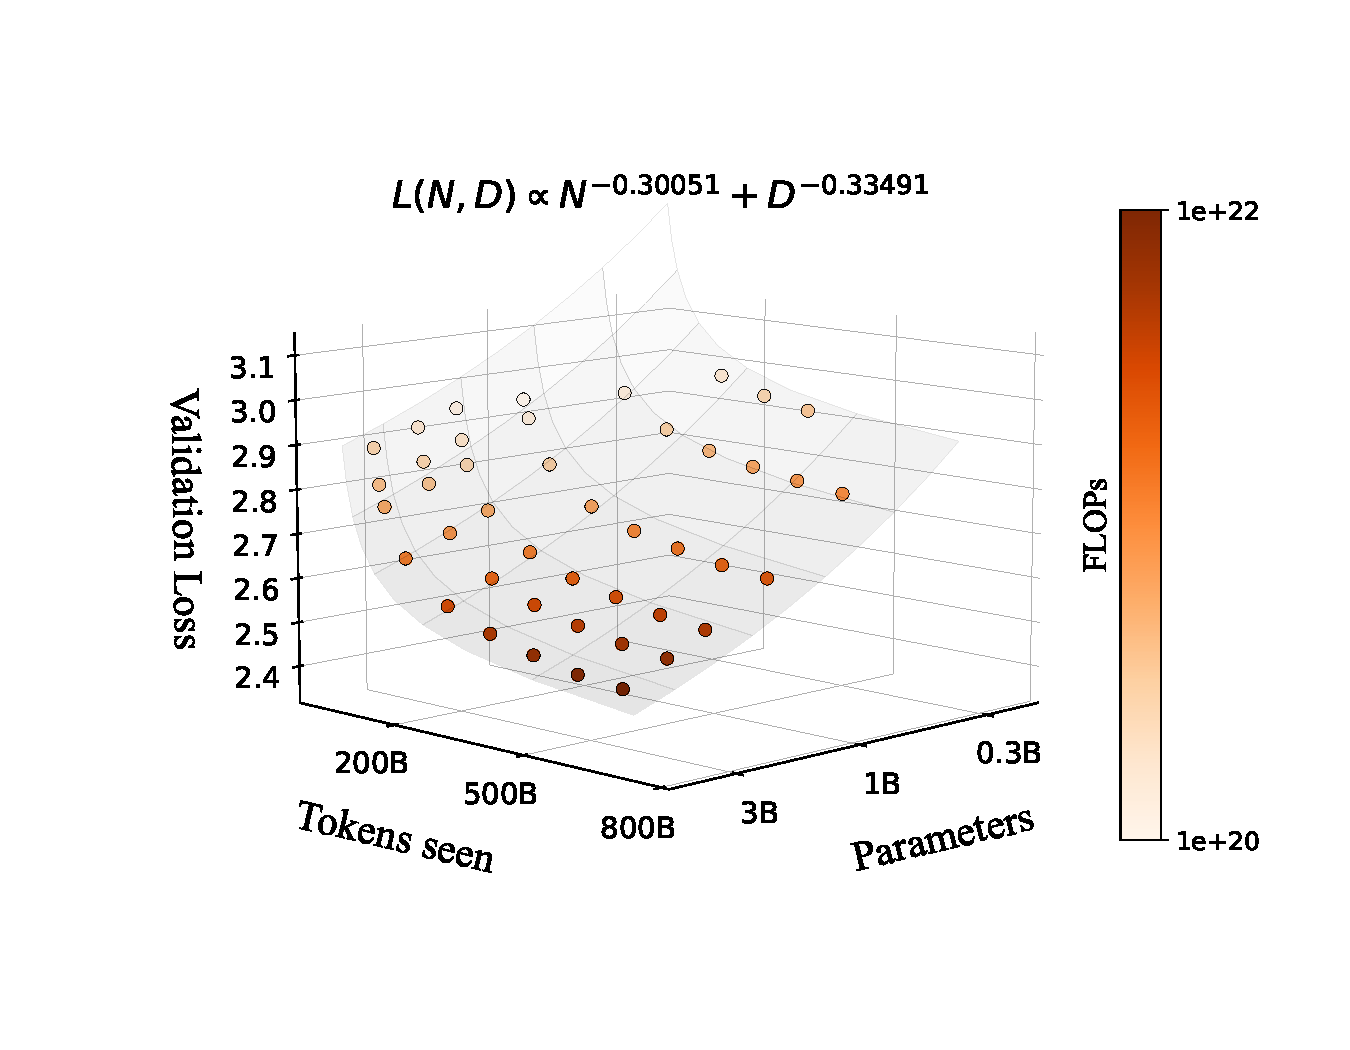
\includegraphics[width=1.02\linewidth]{assets/early/3d_scaling_early.pdf}
    \end{subfigure}
    \hfil
    \begin{subfigure}[t]{0.48\linewidth}
        \centering
        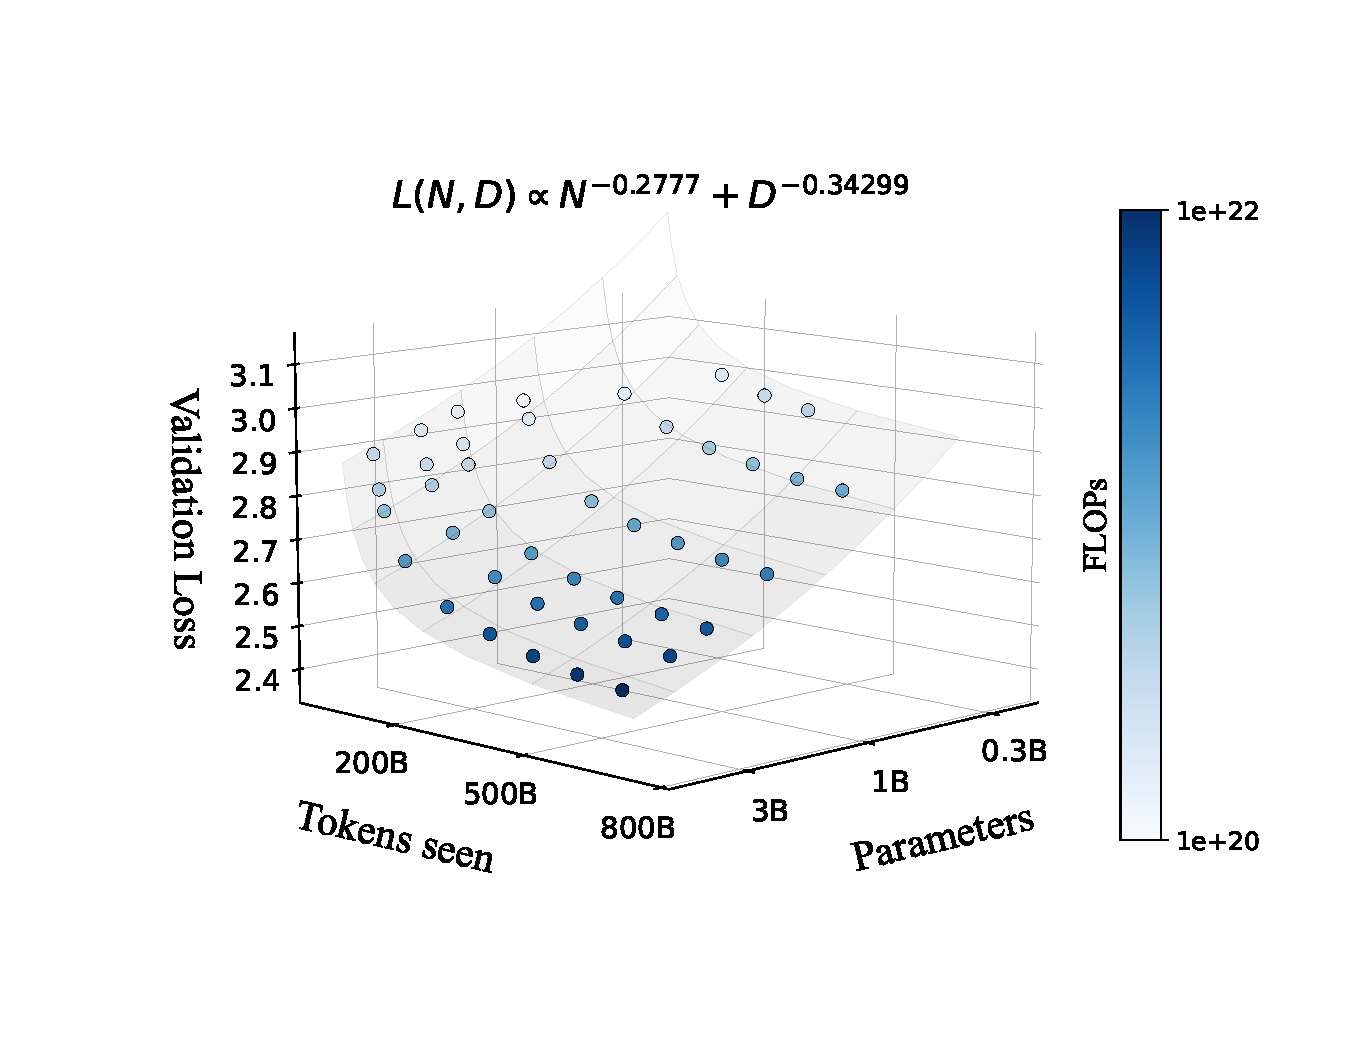
\includegraphics[width=1.02\linewidth]{assets/early/3d_scaling_late.pdf}
    \end{subfigure}
    \vspace{5pt}
    \setlength{\fboxsep}{0.5pt}
    \setlength{\fboxrule}{0pt}
    \caption{\textbf{Scaling laws for \fbox{\colorbox{CustomC_Light1!20}{\strut
    early-fusion}} and \fbox{\colorbox{CustomD_Light1!20}{late-fusion\strut}}
    native multimodal models.} Each point represents a model (300M to 3B
    parameters) trained on varying \edit{number of} tokens (250M to 400B). We
    report the average cross-entropy loss on the validation sets of
    \edit{interleaved (Obelics), Image-caption (HQITP), and text-only data
    (DCLM).}}
    \label{fig:early_vs_late_scaleflops_3d}
\end{figure}
        

\begin{table}[h]
    \centering
    \setlength{\tabcolsep}{16pt}
    \renewcommand{\arraystretch}{1}
    \resizebox{1\linewidth}{!}{
    \begin{tabular}{lccrc}
        Data type & dataset & \#samples & sampling prob. \\
         \shline
         \multirow{3}{*}{Image-Caption} &  DFN~\citep{fang2023data} & 2B & 27\%
         \\
          & COYO~{\citep{kakaobrain2022coyo700m}} &  600M & 11.25\% \\
          & HQITP  & 400M & 6.75\% \\
          Interleaved & Obelics \citep{laurenccon2024obelics}  & 141M Docs &
          45\% \\
          Text & DCLM \citep{li2024datacomp} & 6.6T Toks & 10\% \\
          
    \end{tabular}} \caption{\textbf{Pre-training data mixture.} Unless otherwise
    specified, the training mixture contains 45\%, 45\% and 10\% of image
    captions, interleaved documents and text-only data.}
    \label{tab:pretraining_datasets}
    \vspace{-5pt}
\end{table}

\subsection{Experimental setup}
\edit{Our models} are based on the autoregressive transformer
architecture~\citep{vaswani2017attention} with SwiGLU
FFNs~\citep{shazeer2020glu} and QK-Norm~\citep{dehghani2023scaling}
following~\citet{li2024datacomp}. In early-fusion models, image patches are
linearly projected to match the text token dimension, while late-fusion follows
the CLIP architecture~\citep{radford2021learning}. We adopt causal attention for
text tokens and bidirectional attention for image tokens, we found this to work
better. Training is conducted on a mixture of public and private multimodal
datasets, including DCLM \citep{li2024datacomp}, Obelics
\citep{laurenccon2024obelics}, DFN \citep{fang2023data}, COYO
\citep{kakaobrain2022coyo700m}, and a private collection of High-Quality
Image-Text Pairs (HQITP) (see \cref{tab:pretraining_datasets}). Images are
\edit{resized} to 224×224 resolution with a 14×14 patch size. We use a context
length of 1k for the multimodal sequences. For training efficiency, we train our
models with \texttt{bfloat16},  Fully Sharded Data Parallel (FSDP)
\citep{zhao2023pytorch}, \edit{activation} checkpointing, and gradient accumulation. We
also use sequence packing for the image captioning dataset to reduce the amount
of padded tokens. Similar to previous
works~\citep{hoffmann2022training,aghajanyan2023scalingmm,abnar2025parameters},
we evaluate performance on a held-out subsets of interleaved (Obelics),
Image-caption (HQITP), and text-only data (DCLM). Further implementation details
are provided in~\cref{app:implementation_details}.







 











\section{Scaling  native multimodal models}








In this section, we present a scaling laws study of native multimodal models,
examining various architectural choices~\cref{sec:scaling_laws_early}, exploring
different data mixtures~\cref{sec:scaling_data_mix}, analyzing the practical
trade-offs between late and early fusion
NMMs, and comparing the performance of native
pre-training and continual pre-training of NMMs~\cref{sec:native_vs_continual}.  

\cpar{Setup.} We train models ranging from 0.3B to 4B active parameters,
scaling the width while keeping the depth constant. For smaller training token
budgets, we reduce the warm-up phase to 1K steps while maintaining 5K steps for
larger budgets.  
Following~\citet{hagele2024scaling}, models are trained with a constant learning
rate, followed by a cool-down phase using an inverse square root scheduler. The
cool-down phase spans 20\% of the total steps spent at the constant learning
rate.  To estimate the scaling coefficients in \Cref{eq:scaling_laws}, we apply the
L-BFGS algorithm~\citep{lbfgs} and Huber loss~\citep{Huber1992} (with $\delta =
10^{-3}$), performing a grid search over initialization ranges.  







\begin{table}[h!]
    \begin{minipage}[b]{1\linewidth}
        \centering
        \setlength{\tabcolsep}{24pt}
        \renewcommand{\arraystretch}{1}
        \resizebox{1\linewidth}{!}{
        \begin{tabular}{c c c c c}
             \grayrow $L \propto E+\frac{1}{N^{\alpha}}+\frac{1}{D^{\beta}}$ & $N \propto C^a$ & $D \propto C^b$ & $L \propto C^c$ & $D \propto N^d$ \\
        \end{tabular}}
      \label{tab:power_laws}
      \vspace{-3mm}
    \end{minipage}
    \begin{minipage}[b]{1\linewidth}
        \centering
        \setlength{\tabcolsep}{8pt}
        \renewcommand{\arraystretch}{1}
        \resizebox{1\linewidth}{!}{
        \begin{tabular}{lccccccccc}
            Model & Data & E & $\alpha$ & $\beta$ & a & b  & c & d \\ %
            \shline
            GPT3 \citep{brown2020language} & Text &  -- & -- & -- & -- & -- & -0.048 & \\% & 1.7 \\
            Chinchilla \citep{hoffmann2022training} & Text &  1.693 & 0.339 & 0.285 & 0.46 & 0.54 & -- & \\%& 20 \\
            \midrule
            \multirow{4}{*}{NMM (early-fusion)} & Text &  2.222 & 0.308 & 0.338 & 0.525 & 0.477     & -0.042 & 0.909 \\%& 58.35\\
            & Image-Caption & 1.569 & 0.311 & 0.339 & 0.520 & 0.479 & -0.061 & 0.919 \\% & 72.21\\
            & Interleaved & 1.966 & 0.297 & 0.338 & 0.532 & 0.468     & -0.046 & 0.879 \\%& 57.74\\
            & AVG & 1.904 & 0.301 & 0.335 & 0.526 & 0.473 & -0.049 & 0.899 \\% & 64.05\\
            \midrule
            NMM (late-fusion) & AVG &  1.891 & 0.290 & 0.338 & 0.636 & 0.462 & -0.049 & 0.673 \\%& 46.19\\
            \midrule
            \edit{Sparse NMM (early-fusion)} & AVG & 2.158  & 0.710 & 0.372 & 0.361  & 0.656 & -0.047 & 1.797 \\%& 46.19\\
        \end{tabular}%
        } \caption{\textbf{Scaling laws for native multimodal models}. We report the
        scaling laws results for early and late fusion models. We fit the scaling laws for different target data types as well as their average loss (AVG).
        }
        \label{tab:early_vs_late_coeffs}
    \end{minipage}
    \vspace{-3mm}
\end{table}
       

\begin{figure*}[t!]
    \centering
    \captionsetup{type=figure}
    \begin{subfigure}[t]{0.33\linewidth}
        \begin{tikzpicture}
    \begin{axis}[
        legend pos=north east,
        grid=major, %
        grid style={line width=.1pt, draw=gray!30}, %
        major grid style={line width=.2pt,draw=gray!50},
        minor tick num=2,
        axis x line*=bottom,
        axis y line*=left,
        xmode=log, %
        log basis x=10, %
        height=1.7in,
        width=1.05\linewidth,
        ylabel style={align=center, font=\scriptsize, yshift=-1ex},
        xlabel style={font=\scriptsize},
        ylabel={\footnotesize{Validation Loss}},
        xlabel={\scriptsize{FLOPs}},
        title=\footnotesize{Image-Caption},
        yticklabel style={font=\scriptsize, /pgf/number format/fixed, /pgf/number format/precision=1},
        xticklabel style={font=\scriptsize},
        mark options={solid},
        legend style={cells={align=left}, font=\footnotesize, text=black}, %
        legend columns=6, %
        legend cell align={left},
        legend to name=sharedlegend,
    ]
    \addplot[legend late_0_2b style] plot coordinates {
        (8.1e+19, 2.967)
        (1.62e+20, 2.874)
        (3.24e+20, 2.797)
        (6.48e+20, 2.728)

    };

    \addplot[legend late_0_4b style] plot coordinates {
        (1.37e+20, 2.869)
        (2.74e+20, 2.771)
        (5.48e+20, 2.695)
        (1.1e+21, 2.626)

    };

    \addplot[legend late_0_9b style] plot coordinates {
        (2.78e+20, 2.734)
        (5.56e+20, 2.629)
        (1.11e+21, 2.541)
        (2.22e+21, 2.467)

    };



    \addplot[legend late_2_2b style] plot coordinates {
        (1.34e+21, 2.466)
        (2.69e+21, 2.367)
        (5.37e+21, 2.287)
        (8.06e+21, 2.255)
    };

        







    \addplot[legend early_0_2b style] plot coordinates {
        (8.25e+19, 2.95)
        (1.65e+20, 2.865)
        (3.3e+20, 2.781)
        (6.6e+20, 2.715)


    };
    \addplot[legend early_0_4b style] plot coordinates {
        (1.39e+20, 2.852)
        (2.78e+20, 2.755)
        (5.57e+20, 2.663)
        (1.11e+21, 2.596)


    };
    \addplot[legend early_0_9b style] plot coordinates {
        (2.8e+20, 2.716)
        (5.59e+20, 2.598)
        (1.12e+21, 2.495)
        (2.24e+21, 2.425)


    };

        
    \addplot[legend early_2_2b style] plot coordinates {
        (1.37e+21, 2.455)
        (2.74e+21, 2.352)
        (5.47e+21, 2.279)
        (8.21e+21, 2.242)
    };
        
    

    \end{axis}
\end{tikzpicture}
    \end{subfigure}
    \begin{subfigure}[t]{0.32\linewidth}
        \begin{tikzpicture}
    \begin{axis}[
        legend pos=north east,
        grid=major, %
        grid style={line width=.1pt, draw=gray!30}, %
        major grid style={line width=.2pt,draw=gray!50},
        minor tick num=2,
        axis x line*=bottom,
        axis y line*=left,
        xmode=log, %
        log basis x=10, %
        height=1.7in,
        width=1.05\linewidth,
        ylabel style={align=center, font=\scriptsize, yshift=-1ex},
        xlabel style={font=\scriptsize},
        xlabel={\scriptsize{FLOPs}},
        title=\footnotesize{Interleaved},
        yticklabel style={font=\scriptsize, /pgf/number format/fixed, /pgf/number format/precision=1},
        xticklabel style={font=\scriptsize},
        mark options={solid},
        legend style={cells={align=left}, font=\footnotesize, text=black}, %
        legend columns=6, %
        legend cell align={left},
        legend to name=sharedlegend,
    ]

    
    \addplot[legend late_0_2b style] plot coordinates {
        (8.1e+19, 3.113)
        (1.62e+20, 3.044)
        (3.24e+20, 2.988)
        (4.86e+20, 2.959)
        (6.48e+20, 2.94)
    };

    \addplot[legend late_0_4b style] plot coordinates {
        (1.37e+20, 3.013)
        (2.74e+20, 2.942)
        (5.48e+20, 2.883)
        (8.22e+20, 2.853)
        (1.1e+21, 2.833)

    };

    \addplot[legend late_0_9b style] plot coordinates {
        (2.78e+20, 2.899)
        (5.56e+20, 2.811)
        (1.11e+21, 2.741)
        (2.22e+21, 2.685)

    };
    \addlegendentry{Late-1B}


    \addplot[legend late_2_2b style] plot coordinates {
        (1.34e+21, 2.697)
        (2.69e+21, 2.621)
        (4.03e+21, 2.58)
        (5.37e+21, 2.557)
        (8.06e+21, 2.527)

    };
    \addlegendentry{Late-2.4B}


    \addplot[legend early_0_2b style] plot coordinates {
        (8.25e+19, 3.094)
        (1.65e+20, 3.022)
        (3.3e+20, 2.967)
        (4.95e+20, 2.939)
        (6.6e+20, 2.921)
    };

    \addplot[legend early_0_4b style] plot coordinates {
        (1.39e+20, 2.998)
        (2.78e+20, 2.927)
        (5.57e+20, 2.866)
        (8.35e+20, 2.836)
        (1.11e+21, 2.817)
    };

    \addplot[legend early_0_9b style] plot coordinates {
        (2.8e+20, 2.885)
        (5.59e+20, 2.795)
        (1.12e+21, 2.726)
        (2.24e+21, 2.669)
    };

    \addlegendentry{Early-0.9B}


    \addplot[legend early_2_2b style] plot coordinates {
        (1.37e+21, 2.685)
        (2.74e+21, 2.61)
        (4.1e+21, 2.572)
        (5.47e+21, 2.542)
        (8.21e+21, 2.514)
              
    };
    \addlegendentry{Early-2.2B}

           


    \end{axis}
\end{tikzpicture}
    \end{subfigure}
    \begin{subfigure}[t]{0.32\linewidth}
        
\begin{tikzpicture}
    \begin{axis}[
        legend pos=north east,
        grid=major, %
        grid style={line width=.1pt, draw=gray!30}, %
        major grid style={line width=.2pt,draw=gray!50},
        minor tick num=2,
        axis x line*=bottom,
        axis y line*=left,
        xmode=log, %
        log basis x=10, %
        height=1.7in,
        width=1.05\linewidth,
        ylabel style={align=center, font=\scriptsize, yshift=-1ex},
        xlabel style={font=\scriptsize},
        xlabel={\scriptsize{FLOPs}},
        title=\footnotesize{Text-only},
        yticklabel style={font=\scriptsize, /pgf/number format/fixed, /pgf/number format/precision=1},
        xticklabel style={font=\scriptsize},
        mark options={solid},
        legend style={cells={align=left}, font=\scriptsize, text=black}, %
        legend columns=4, %
        legend cell align={left},
        legend to name=sharedlegend,
    ]

    \addplot[legend late_0_2b style] plot coordinates {
        (8.1e+19, 3.349)
        (1.62e+20, 3.281)
        (3.24e+20, 3.226)
        (4.86e+20, 3.197)
        (6.48e+20, 3.179)

    };
    \addlegendentry{Late-289M}

    \addplot[legend late_0_4b style] plot coordinates {
        (1.37e+20, 3.249)
        (2.74e+20, 3.177)
        (5.48e+20, 3.12)
        (8.22e+20, 3.09)
        (1.1e+21, 3.071)
    };
    \addlegendentry{Late-494M}


    \addplot[legend late_0_9b style] plot coordinates {
        (2.78e+20, 3.134)
        (5.56e+20, 3.045)
        (1.11e+21, 2.976)
        (1.67e+21, 2.941)
        (2.22e+21, 2.92)

    };
    \addlegendentry{Late-1B}



    \addplot[legend late_2_2b style] plot coordinates {
        (1.34e+21, 2.936)
        (2.69e+21, 2.859)
        (5.37e+21, 2.798)
        (8.06e+21, 2.765)
        
    };
    \addlegendentry{Late-2.4B}



    
        




    \addplot[legend early_0_2b style] plot coordinates {
        (8.25e+19, 3.328)
        (1.65e+20, 3.259)
        (3.3e+20, 3.203)
        (4.95e+20, 3.175)
        (6.6e+20, 3.157)
    };
    \addlegendentry{Early-275M}



    \addplot[legend early_0_4b style] plot coordinates {
        (1.39e+20, 3.232)
        (2.78e+20, 3.161)
        (5.57e+20, 3.103)
        (8.35e+20, 3.073)
        (1.11e+21, 3.054)
    };
    \addlegendentry{Early-464M}

    \addplot[legend early_0_9b style] plot coordinates {
        (2.8e+20, 3.119)
        (5.59e+20, 3.03)
        (1.12e+21, 2.961)
        (1.68e+21, 2.926)
        (2.24e+21, 2.904)
    };
    \addlegendentry{Early-932M}


        

    \addplot[legend early_2_2b style] plot coordinates {
        (1.37e+21, 2.923)
        (2.74e+21, 2.846)
        (5.47e+21, 2.784)
        (8.21e+21, 2.752)
    };
    \addlegendentry{Early-2.28B}


        
    

    \end{axis}
\end{tikzpicture}
    \end{subfigure}
    \begin{center}
        \ref{sharedlegend}
    \end{center}
    \caption{\textbf{Early vs late fusion: scaling training FLOPs.} We compare
    early and late fusion models when scaling both the number of model parameters and the number
    of training tokens. Overall, early fusion shows a slight advantage, especially at smaller model sizes, and the gap decreases when scaling the number of parameters $N$.}
    \label{fig:early_vs_late_scaleflops}
    \vspace{3mm}
\end{figure*}




\vspace{-0.5cm}
\subsection{Scaling laws of NMMs}
\label{sec:scaling_laws_early}

\cpar{Scaling laws for early-fusion and late-fusion models.}  
\Cref{fig:early_vs_late_scaleflops_3d}~(left) presents the final loss averaged
across interleaved, image-caption, and text datasets for early-fusion NMMs. The
lowest-loss frontier follows a power law as a function of FLOPs. Fitting the
power law yields the expression $L \propto C^{-0.049}$, indicating the rate of
improvement with increasing compute. When analyzing the scaling laws per data
type (\eg, image-caption, interleaved, text), we observe that the exponent
varies (\cref{tab:early_vs_late_coeffs}). For instance, the model achieves a
higher rate of improvement for image-caption data $(L \propto C^{-0.061})$ when
compared to interleaved documents $(L \propto C^{-0.046}$).  

To model the loss as a function of the number of training tokens $D$ and model
parameters $N$, we fit the parametric function in \cref{eq:scaling_laws}, obtaining
scaling exponents $\alpha = 0.301$ and $\beta = 0.335$. These describe the rates
of improvement when scaling the number of model parameters and training tokens, respectively.
Assuming a linear relationship between compute, $N$, and $D$ (\ie, $C \propto ND$),
we derive the law relating model parameters to the compute budget (see
\cref{app:scaling_laws} for details). Specifically, for a given compute budget
$C$, we compute the corresponding model size $N$ at logarithmically spaced $D$
values and determine $N_{opt}$, the parameter count that minimizes loss.
Repeating this across different FLOPs values produces a dataset of $(C,
N_{opt})$, to which we fit a power law predicting the compute-optimal model size
as a function of compute: $N^* \propto C^{0.526}.$

Similarly, we fit power laws to estimate the compute-optimal training dataset
size as a function of compute and model size:  
\[
D_{opt} \propto C^{0.473}, \quad D_{opt} \propto N^{0.899}.
\]  
These relationships allow practitioners to determine the optimal model and
dataset size given a fixed compute budget. When analyzing by data type, we find
that interleaved data benefits more from larger models ($a=0.532$) compared to
image-caption data ($a=0.520$), whereas the opposite trend holds for training
tokens.  






\begin{figure*}[t!]
    \centering
    \captionsetup{type=figure}
    \begin{subfigure}[t]{0.24\linewidth}
        \begin{tikzpicture}
    \begin{axis}[
        grid=both,
        grid style={line width=.1pt, draw=gray!10},
        major grid style={line width=.2pt,draw=gray!50},
        minor tick num=2,
        axis x line*=bottom,
        axis y line*=left,
        xmode=log, %
        log basis x=10, %
        xtick={
            1E+19,
            1E+20,
            1E+21,
            1E+22
        },
        xmin=2E+18,
        xmax=2E+22,
        ymax=4.3,
        height=1.7in,
        width=1.15\linewidth,
        ylabel style={align=center, font=\scriptsize, yshift=-1ex},
        xlabel style={font=\scriptsize},
        title={\footnotesize{\colorbox{blue!10}{45-45-10}}},
        ylabel={Validation Loss},
        xlabel={\scriptsize{FLOPs}},
        yticklabel style={font=\scriptsize},
        xticklabel style={font=\scriptsize},
        legend style={cells={align=left}, font=\scriptsize, fill opacity=0.7, fill=none,at={(-0.3,0.95)}, anchor=west, draw=none}, %
        legend cell align={left},
        mark options={solid},
    ]


    \addplot[color=white, samples=50, domain=5e18:10e21, mark=none] {29.574*x^(-0.04919)};
    \addlegendentry{\scalebox{0.9}{$L = 29.574C^{-0.0492}$}};
    \addplot[color=black, samples=50, domain=5e18:10e21, forget plot] {29.574*x^(-0.04919)};


    

    
    



    \addplot[legend early_0_2b style, mark size=1pt] plot coordinates {
        (4.13e+18, 3.9896666666666665)
        (8.25e+18, 3.5996666666666663)
        (1.24e+19, 3.468)
        (2.06e+19, 3.358333333333333)
        (4.13e+19, 3.2113333333333336)
        (6.19e+19, 3.1543333333333337)
        (8.25e+19, 3.124)
        (1.65e+20, 3.048666666666667)
        (3.3e+20, 2.9836666666666667)
        (4.95e+20, 2.9506666666666668)
        (6.6e+20, 2.9309999999999996)
    };
    \addplot[legend early_0_4b style, mark size=1pt] plot coordinates {
        (6.96e+18, 3.887333333333333)
        (1.39e+19, 3.5203333333333333)
        (2.09e+19, 3.3823333333333334)
        (3.48e+19, 3.2710000000000004)
        (6.96e+19, 3.1170000000000004)
        (1.04e+20, 3.058666666666667)
        (1.39e+20, 3.0273333333333334)
        (2.78e+20, 2.9476666666666667)
        (5.57e+20, 2.877333333333333)
        (8.35e+20, 2.8433333333333333)
        (1.11e+21, 2.8223333333333334)
        (1.39e+21, 2.8063333333333333)
        (1.67e+21, 2.7936666666666667)
    };
    \addplot[legend early_0_9b style, mark size=1pt] plot coordinates {
        (1.4e+19, 3.955)
        (2.8e+19, 3.465)
        (4.19e+19, 3.3143333333333334)
        (6.99e+19, 3.2099999999999995)
        (1.4e+20, 3.0193333333333334)
        (2.1e+20, 2.9483333333333337)
        (2.8e+20, 2.9066666666666663)
        (5.59e+20, 2.807666666666666)
        (1.12e+21, 2.7273333333333327)
        (1.68e+21, 2.688333333333333)
        (2.24e+21, 2.666)
        (2.8e+21, 2.6466666666666665)
        (3.36e+21, 2.635333333333333)
    };

    \addplot[legend early style, mark size=1pt] plot coordinates {
        (2.44e+19, 3.859666666666667)
        (4.88e+19, 3.3973333333333335)
        (7.32e+19, 3.25)
        (1.22e+20, 3.1323333333333334)
        (2.44e+20, 2.9466666666666668)
        (3.66e+20, 2.875666666666667)
        (4.88e+20, 2.8206666666666664)
        (9.76e+20, 2.7246666666666672)
        (1.95e+21, 2.646666666666667)
        (2.93e+21, 2.6056666666666666)
        (3.9e+21, 2.582333333333333)
        (4.88e+21, 2.562)
        (5.86e+21, 2.548666666666666)
    };

    \addplot[legend early_2_2b style, mark size=1pt] plot coordinates {
        (3.42e+19, 3.859666666666667)
        (6.84e+19, 3.3973333333333335)
        (1.03e+20, 3.2503333333333333)
        (1.71e+20, 3.098333333333333)
        (3.42e+20, 2.9156666666666666)
        (5.13e+20, 2.8396666666666666)
        (6.84e+20, 2.7913333333333337)
        (1.37e+21, 2.687666666666667)
        (2.74e+21, 2.6026666666666665)
        (4.1e+21, 2.562)
        (5.47e+21, 2.5349999999999997)
        (6.84e+21, 2.5146666666666664)
        (8.21e+21, 2.502666666666667)
    };
    \addplot[legend early_3_3b style, mark size=1pt] plot coordinates {
        (5.03e+19, 3.746333333333333)
        (1.01e+20, 3.324)
        (1.51e+20, 3.1786666666666665)
        (2.52e+20, 3.0766666666666667)
        (5.03e+20, 2.8836666666666666)
        (7.55e+20, 2.8029999999999995)
        (1.01e+21, 2.7550000000000003)
        (2.01e+21, 2.6473333333333335)
        (4.02e+21, 2.5583333333333336)
        (6.04e+21, 2.5163333333333333)
        (8.05e+21, 2.4886666666666666)
        (1.01e+22, 2.466666666666667)
    };
    

    \end{axis}
\end{tikzpicture}
    \end{subfigure}
    \begin{subfigure}[t]{0.24\linewidth}
        
\begin{tikzpicture}
    \begin{axis}[
        legend pos=north east,
        grid=both,
        grid style={line width=.1pt, draw=gray!10},
        major grid style={line width=.2pt,draw=gray!50},
        minor tick num=2,
        axis x line*=bottom,
        axis y line*=left,
        xmode=log, %
        log basis x=10, %
        xtick={
            1E+19,
            1E+20,
            1E+21,
            1E+22
        },
        xmin=2E+18,
        xmax=2E+22,
        ymax=4.3,
        height=1.7in,
        width=1.15\linewidth,
        ylabel style={align=center, font=\scriptsize, yshift=-1ex},
        xlabel style={font=\scriptsize},
        title=\footnotesize{\colorbox{green!10}{40-20-40}},
        xlabel={\scriptsize{FLOPs}},
        yticklabel style={font=\scriptsize},
        xticklabel style={font=\scriptsize},
        legend style={cells={align=left}, font=\scriptsize, fill opacity=0.7, fill=none,  draw=none,at={(-0.3,0.95)}, anchor=west}, %
        legend cell align={left},
        mark options={solid},
    ]

    \addplot[color=white, samples=50, domain=5e18:10e21, mark=none] {29.574*x^(-0.04919)};
    \addlegendentry{\scalebox{0.9}{$L = 28.590C^{-0.0486}$}};
    \addplot[color=black, samples=50, domain=5e18:10e21] {28.589490029895153*x^(-0.048605069004824725)};

    \addplot[legend early_0_2b style, mark size=1pt] plot coordinates {
        (4.13e+18, 3.968)
        (8.25e+18, 3.563)
        (1.24e+19, 3.4296666666666664)
        (2.06e+19, 3.3236666666666665)
        (4.13e+19, 3.203)
        (6.19e+19, 3.1486666666666667)
        (8.25e+19, 3.1169999999999995)
        (1.65e+20, 3.0446666666666666)
        (3.3e+20, 2.9906666666666673)
        (4.95e+20, 2.9633333333333334)
        (6.6e+20, 2.9456666666666664)
    };
    \addplot[legend early_0_4b style, mark size=1pt] plot coordinates {
        (6.96e+18, 3.8580000000000005)
        (1.39e+19, 3.471)
        (2.09e+19, 3.3443333333333336)
        (3.48e+19, 3.2196666666666665)
        (6.96e+19, 3.097666666666667)
        (1.04e+20, 3.0393333333333334)
        (1.39e+20, 3.011333333333333)
        (2.78e+20, 2.935333333333333)
        (5.57e+20, 2.871)
        (8.35e+20, 2.8386666666666667)
        (1.11e+21, 2.8190000000000004)
        (1.39e+21, 2.8030000000000004)
        (1.67e+21, 2.7913333333333337)
    };
    \addplot[legend early_0_9b style, mark size=1pt] plot coordinates {
        (1.4e+19, 3.9250000000000003)
        (2.8e+19, 3.426666666666667)
        (4.19e+19, 3.2733333333333334)
        (6.99e+19, 3.1326666666666667)
        (1.4e+20, 2.9979999999999998)
        (2.1e+20, 2.9246666666666665)
        (2.8e+20, 2.8943333333333334)
        (5.59e+20, 2.8070000000000004)
        (1.12e+21, 2.7283333333333335)
        (1.68e+21, 2.6886666666666668)
        (2.24e+21, 2.666)
        (2.8e+21, 2.6476666666666664)
        (3.36e+21, 2.636)
    };

    \addplot[legend early style, mark size=1pt] plot coordinates {
        (2.44e+19, 3.846)
        (4.88e+19, 3.3570000000000007)
        (7.32e+19, 3.207333333333333)
        (1.22e+20, 3.0636666666666668)
        (2.44e+20, 2.9229999999999996)
        (3.66e+20, 2.848666666666667)
        (4.88e+20, 2.8166666666666664)
        (9.76e+20, 2.7126666666666672)
        (1.95e+21, 2.632)
        (2.93e+21, 2.592333333333333)
        (3.9e+21, 2.569666666666667)
        (4.88e+21, 2.5516666666666667)
        (5.86e+21, 2.538)
    };

    \addplot[legend early_2_2b style, mark size=1pt] plot coordinates {
        (3.42e+19, 3.771333333333333)
        (6.84e+19, 3.317)
        (1.03e+20, 3.1679999999999997)
        (1.71e+20, 3.025)
        (3.42e+20, 2.887)
        (5.13e+20, 2.8106666666666666)
        (6.84e+20, 2.781333333333334)
        (1.37e+21, 2.6756666666666664)
        (2.74e+21, 2.593666666666666)
        (4.1e+21, 2.5526666666666666)
        (5.47e+21, 2.526666666666667)
        (6.84e+21, 2.5093333333333336)
        (8.21e+21, 2.494333333333333)
    };
    \addplot[legend early_3_3b style, mark size=1pt] plot coordinates {
        (5.03e+19, 3.7276666666666665)
        (1.01e+20, 3.2793333333333337)
        (1.51e+20, 3.1359999999999997)
        (2.52e+20, 2.9949999999999997)
        (5.03e+20, 2.879)
        (7.55e+20, 2.787333333333333)
        (1.01e+21, 2.738666666666667)
        (2.01e+21, 2.6276666666666664)
        (4.02e+21, 2.5466666666666664)
        (6.04e+21, 2.5180000000000002)
        (8.05e+21, 2.4789999999999996)
        (1.01e+22, 2.456)
        (1.21e+22, 2.4516666666666667)
    };
    

    \end{axis}
\end{tikzpicture}
    \end{subfigure}
    \begin{subfigure}[t]{0.24\linewidth}
        
\begin{tikzpicture}
    \begin{axis}[
        legend pos=north east,
        grid=both,
        grid style={line width=.1pt, draw=gray!10},
        major grid style={line width=.2pt,draw=gray!50},
        minor tick num=2,
        axis x line*=bottom,
        axis y line*=left,
        xmode=log, %
        log basis x=10, %
        xtick={
            1E+19,
            1E+20,
            1E+21,
            1E+22
        },
        xmin=2E+18,
        xmax=2E+22,
        ymax=4.3,
        height=1.7in,
        width=1.15\linewidth,
        ylabel style={align=center, font=\scriptsize, yshift=-1ex},
        xlabel style={font=\scriptsize},
        title=\footnotesize{\colorbox{red!10}{30-30-40}},
        xlabel={\scriptsize{FLOPs}},
        yticklabel style={font=\scriptsize},
        xticklabel style={font=\scriptsize},
        legend style={cells={align=left}, font=\scriptsize, fill opacity=0.7, fill=none,  draw=none,at={(-0.3,0.95)}, anchor=west}, %
        legend cell align={left},
        mark options={solid},
    ]

    \addplot[color=white, samples=50, domain=5e18:10e21, mark=none] {29.574*x^(-0.04919)};
    \addlegendentry{\scalebox{0.9}{$L = 25.623C^{-0.0463}$}};
    \addplot[color=black, samples=50, domain=5e18:10e21] {25.622649599876997*x^(-0.04634327762259929)};

    \addplot[legend early_0_2b style, mark size=1pt] plot coordinates {
        (4.13e+18, 3.9586666666666672)
        (8.25e+18, 3.568)
        (1.24e+19, 3.402333333333333)
        (2.06e+19, 3.235666666666667)
        (4.13e+19, 3.200333333333333)
        (6.19e+19, 3.1493333333333333)
        (8.25e+19, 3.0506666666666664)
        (1.65e+20, 2.9996666666666663)
        (3.3e+20, 2.9996666666666663)
        (4.95e+20, 2.969666666666667)
        (6.6e+20, 2.9486666666666665)
    };
    \addplot[legend early_0_4b style, mark size=1pt] plot coordinates {
        (6.96e+18, 3.8503333333333334)
        (1.39e+19, 3.472)
        (2.09e+19, 3.3366666666666664)
        (3.48e+19, 3.2273333333333336)
        (6.96e+19, 3.095)
        (1.04e+20, 3.0406666666666666)
        (1.39e+20, 3.016)
        (2.78e+20, 2.9373333333333336)
        (5.57e+20, 2.8753333333333337)
        (8.35e+20, 2.8433333333333333)
        (1.11e+21, 2.8223333333333334)
        (1.39e+21, 2.8073333333333337)
        (1.67e+21, 2.797333333333333)
    };
    \addplot[legend early_0_9b style, mark size=1pt] plot coordinates {
        (1.4e+19, 3.8346666666666667)
        (2.8e+19, 3.3586666666666662)
        (4.19e+19, 3.202)
        (6.99e+19, 3.1340000000000003)
        (1.4e+20, 2.9949999999999997)
        (2.1e+20, 2.9273333333333333)
        (2.8e+20, 2.8930000000000002)
        (5.59e+20, 2.8053333333333335)
        (1.12e+21, 2.728333333333333)
        (1.68e+21, 2.692666666666667)
        (2.24e+21, 2.667666666666667)
        (2.8e+21, 2.6496666666666666)
        (3.36e+21, 2.639666666666667)
    };

    \addplot[legend early style, mark size=1pt] plot coordinates {
        (2.44e+19, 3.8346666666666667)
        (4.88e+19, 3.3586666666666662)
        (7.32e+19, 3.202)
        (1.22e+20, 3.063333333333334)
        (2.44e+20, 2.9196666666666666)
        (3.66e+20, 2.8503333333333334)
        (4.88e+20, 2.8196666666666665)
        (9.76e+20, 2.719)
        (1.95e+21, 2.6359999999999997)
        (2.93e+21, 2.6)
        (3.9e+21, 2.574)
        (4.88e+21, 2.554)
        (5.86e+21, 2.5436666666666667)
    };

    \addplot[legend early_2_2b style, mark size=1pt] plot coordinates {
        (3.42e+19, 3.755333333333333)
        (6.84e+19, 3.311)
        (1.03e+20, 3.159333333333333)
        (1.71e+20, 3.025)
        (3.42e+20, 2.8770000000000002)
        (5.13e+20, 2.8089999999999997)
        (6.84e+20, 2.781333333333333)
        (1.37e+21, 2.679)
        (2.74e+21, 2.595)
        (4.1e+21, 2.5536666666666665)
        (5.47e+21, 2.5283333333333333)
        (6.84e+21, 2.5066666666666664)
        (8.21e+21, 2.4953333333333334)
    };
    \addplot[legend early_3_3b style, mark size=1pt] plot coordinates {
        (5.03e+19, 3.7100000000000004)
        (1.01e+20, 3.276666666666667)
        (1.51e+20, 3.1300000000000003)
        (2.52e+20, 2.997)
        (5.03e+20, 2.84)
        (7.55e+20, 2.768333333333333)
        (1.01e+21, 2.7436666666666665)
        (2.01e+21, 2.6343333333333336)
        (4.02e+21, 2.5513333333333335)
        (6.04e+21, 2.5086666666666666)
        (8.05e+21, 2.483)
        (1.01e+22, 2.4616666666666664)
    };
    

    \end{axis}
\end{tikzpicture}
    \end{subfigure}
    \begin{subfigure}[t]{0.24\linewidth}
        
\begin{tikzpicture}
    \begin{axis}[
        legend pos=north east,
        grid=both,
        grid style={line width=.1pt, draw=gray!10},
        major grid style={line width=.2pt,draw=gray!50},
        minor tick num=2,
        axis x line*=bottom,
        axis y line*=left,
        xmode=log, %
        log basis x=10, %
        xtick={
            1E+19,
            1E+20,
            1E+21,
            1E+22
        },
        xmin=2E+18,
        xmax=2E+22,
        ymax=4.3,
        height=1.7in,
        width=1.15\linewidth,
        ylabel style={align=center, font=\scriptsize, yshift=-1ex},
        xlabel style={font=\scriptsize},
        title={\footnotesize{\colorbox{orange!10}{20-40-40}}},
        xlabel={\scriptsize{FLOPs}},
        yticklabel style={font=\scriptsize},
        xticklabel style={font=\scriptsize},
        legend style={cells={align=left}, font=\scriptsize, fill opacity=0.7, fill=none,  draw=none,at={(-0.3,0.95)}, anchor=west}, %
        legend cell align={left},
        mark options={solid},
    ]

    \addplot[color=white, samples=50, domain=5e18:10e21, mark=none] {29.574*x^(-0.04919)};
    \addlegendentry{\scalebox{0.9}{$L = 29.002C^{-0.0488}$}};
    \addplot[color=black, samples=50, domain=5e18:10e21] {29.002272950965768*x^(-0.04878835579770303)};

    \addplot[legend early_0_2b style, mark size=1pt] plot coordinates {
        (4.13e+18, 3.984666666666667)
        (8.25e+18, 3.592333333333334)
        (1.24e+19, 3.453333333333333)
        (2.06e+19, 3.3553333333333337)
        (4.13e+19, 3.2129999999999996)
        (6.19e+19, 3.1616666666666666)
        (8.25e+19, 3.1376666666666666)
        (1.65e+20, 3.0653333333333332)
        (3.3e+20, 3.0080000000000005)
        (4.95e+20, 2.9793333333333334)
        (6.6e+20, 2.9603333333333333)
    };
    \addplot[legend early_0_4b style, mark size=1pt] plot coordinates {
        (6.96e+18, 3.861333333333333)
        (1.39e+19, 3.4956666666666667)
        (2.09e+19, 3.361333333333333)
        (3.48e+19, 3.2516666666666665)
        (6.96e+19, 3.1056666666666666)
        (1.04e+20, 3.0546666666666664)
        (1.39e+20, 3.0293333333333337)
        (2.78e+20, 2.959)
        (5.57e+20, 2.9013333333333335)
        (8.35e+20, 2.8683333333333336)
        (1.11e+21, 2.8463333333333334)
        (1.39e+21, 2.8303333333333334)
        (1.67e+21, 2.8193333333333332)
    };
    \addplot[legend early_0_9b style, mark size=1pt] plot coordinates {
        (1.4e+19, 3.936666666666667)
        (2.8e+19, 3.449333333333333)
        (4.19e+19, 3.2886666666666664)
        (6.99e+19, 3.177666666666667)
        (1.4e+20, 3.0066666666666664)
        (2.1e+20, 2.937)
        (2.8e+20, 2.9153333333333333)
        (5.59e+20, 2.8193333333333332)
        (1.12e+21, 2.7426666666666666)
        (1.68e+21, 2.7063333333333333)
        (2.24e+21, 2.6809999999999996)
        (2.8e+21, 2.6626666666666665)
        (3.36e+21, 2.6533333333333338)
    };

    \addplot[legend early style, mark size=1pt] plot coordinates {
        (2.44e+19, 3.8456666666666663)
        (4.88e+19, 3.3783333333333334)
        (7.32e+19, 3.2193333333333336)
        (1.22e+20, 3.1056666666666666)
        (2.44e+20, 2.9299999999999997)
        (3.66e+20, 2.8626666666666662)
        (4.88e+20, 2.834)
        (9.76e+20, 2.731333333333333)
        (1.95e+21, 2.651333333333333)
        (2.93e+21, 2.611333333333333)
        (3.9e+21, 2.590333333333333)
        (4.88e+21, 2.568)
        (5.86e+21, 2.553666666666667)
    };

    \addplot[legend early_2_2b style, mark size=1pt] plot coordinates {
        (3.42e+19, 3.7680000000000002)
        (6.84e+19, 3.3303333333333334)
        (1.03e+20, 3.1780000000000004)
        (1.71e+20, 3.06)
        (3.42e+20, 2.89)
        (5.13e+20, 2.817)
        (6.84e+20, 2.7896666666666667)
        (1.37e+21, 2.685)
        (2.74e+21, 2.6020000000000003)
        (4.1e+21, 2.5646666666666667)
        (5.47e+21, 2.5420000000000003)
        (6.84e+21, 2.5226666666666664)
        (8.21e+21, 2.513666666666667)
    };
    \addplot[legend early_3_3b style, mark size=1pt] plot coordinates {
        (5.03e+19, 3.720333333333334)
        (1.01e+20, 3.2953333333333332)
        (1.51e+20, 3.1453333333333333)
        (2.52e+20, 3.0276666666666667)
        (5.03e+20, 2.8523333333333336)
        (7.55e+20, 2.7756666666666674)
        (1.01e+21, 2.753)
        (2.01e+21, 2.6413333333333333)
        (4.02e+21, 2.558666666666667)
        (6.04e+21, 2.514666666666667)
        (8.05e+21, 2.4883333333333337)
        (1.01e+22, 2.466333333333333)
        (1.21e+22, 2.454333333333333)
    };


    \end{axis}
\end{tikzpicture}
    \end{subfigure}
    \begin{tikzpicture}
        \node[anchor=north] (legend) at (0\linewidth, 0) {
            \begin{axis}[
                        hide axis, %
                        xmin=0, xmax=0.5, ymin=0, ymax=1, %
                        legend columns=6, %
                        legend style={
                            at={(-0.12, 0.05)}, %
                            anchor=north, %
                            /tikz/every even column/.append style={column sep=0.2cm}, %
                            scale=0.5,
                            cells={align=left}, font=\scriptsize,
                            anchor=center,
                        },
                    ]
                \addlegendimage{legend early_0_2b style}
                \addlegendentry{0.275B}
                \addlegendimage{legend early_0_4b style}
                \addlegendentry{0.464B}
                \addlegendimage{legend early_0_9b style}
                \addlegendentry{0.932B}
                \addlegendimage{legend early style}
                \addlegendentry{1.627B}
                \addlegendimage{legend early_2_2b style}
                \addlegendentry{2.280B}
                \addlegendimage{legend early_3_3b style}
                \addlegendentry{3.354B}
            \end{axis}
        };
    \end{tikzpicture}
    \caption{\textbf{Scaling laws with different training mixtures.}
    Early-fusion models follow similar scaling trends when changing the pretraining mixtures. However, increasing the image captions leads to a higher scaling exponent norm (see~\cref{tab:scaling_laws_coeffs_data_mixtures}). 
    }
    \label{fig:early_scaleflops_data_mixtures}
\end{figure*}



We conduct a similar study on late-fusion models
in~\cref{fig:early_vs_late_scaleflops_3d}~(right) and observe comparable scaling
behaviors. In particular, the loss scaling exponent ($c = -0.0494$) is nearly
identical to that of early fusion ($c = -0.0492$).  
This trend is evident in \cref{fig:early_vs_late_scaleflops}, where early fusion
outperforms late fusion at smaller model scales, while both architectures
converge to similar performance at larger model sizes. We also observe similar
trends when varying late-fusion configurations, such as using a smaller vision
encoder with a larger text decoder~\cref{app:late_vs_early}.


\begin{figure}[t!]
    \begin{minipage}[t]{0.48\textwidth}
            \centering
    \captionsetup{type=figure}
    \begin{subfigure}[t]{0.49\linewidth}
        \begin{tikzpicture}
    \begin{axis}[
        ybar,
        bar width=20pt, %
        enlarge x limits=0.4,
        legend pos=north east,
        grid=both,
        grid style={line width=.1pt, draw=gray!10},
        major grid style={line width=.2pt,draw=gray!50},
        axis x line*=bottom,
        axis y line*=left,
        xtick={
            2,
            4,
            6
        },
        height=1.7in,
        width=1.2\linewidth,
        ylabel style={align=center, font=\footnotesize, yshift=-1ex},
        xlabel style={font=\footnotesize},
        title={\footnotesize{Relative Memory Usage}},
        ylabel={\footnotesize{GB per GPU}},
        xlabel={\footnotesize{FLOPs ($\times10^{21}$)}},
        yticklabel style={font=\footnotesize},
        xticklabel style={font=\footnotesize},
        legend style={cells={align=left}, font=\footnotesize, fill opacity=0.7, at={(0.6,0.25)}},
        legend cell align={left},
        ymin=-10,
        ymax=2,
        extra y ticks={0.03},
        extra y tick labels={},
        extra y tick style={grid=major, major grid style={line width=2pt, draw=LateColor, dashed}},
    ]
        \addplot[legend early bars style] coordinates {
            (2,-3.05)
            (4,-5.38)
            (6,-7.59)
        };
        \addlegendentry{Early}
        \node[anchor=west, font=\footnotesize, text=LateColor] at (axis cs:0.4,0.8) {Late};
    \end{axis}
    \end{tikzpicture}
    \end{subfigure}
    \begin{subfigure}[t]{0.49\linewidth}
        
\begin{tikzpicture}
    \begin{axis}[
        ybar, %
        bar width=16pt, %
        enlarge x limits=0.4, %
        legend pos=north east,
        grid=both,
        grid style={line width=.1pt, draw=gray!10},
        major grid style={line width=.2pt,draw=gray!50},
        axis x line*=bottom,
        axis y line*=left,
        xtick={
            2,
            4,
            6
        },
        height=1.7in,
        width=1.2\linewidth,
        ylabel style={align=center, font=\footnotesize, yshift=-1ex},
        xlabel style={font=\footnotesize},
        title={\footnotesize{Relative Train time}},
        ylabel={\footnotesize{Hours}},
        xlabel={\footnotesize{FLOPs ($\times10^{21}$)}},
        yticklabel style={font=\footnotesize},
        xticklabel style={font=\footnotesize},
        legend style={cells={align=left}, font=\footnotesize, fill opacity=0.7, at={(0.6, 0.25)}},
        legend cell align={left},
        ymin=-160,               %
        ymax=32,
        extra y ticks={1},
        extra y tick labels={},
        extra y tick style={grid=major, major grid style={line width=2pt, draw=LateColor, dashed}},
    ]

    \addplot[legend early bars style] coordinates {
        (2, -26)
        (4, -106)
        (6, -123)
    };
    \addlegendentry{Early}

    \node[anchor=west, font=\footnotesize, text=LateColor] at (axis cs:0.1,13) {Late};

    \end{axis}
\end{tikzpicture}

    \end{subfigure}
    \vspace{-3pt}
    \caption{\textbf{Early vs late: pretraining efficiency.} Early-fusion is faster to train and consumes less memory. Models are trained on 16 H100 GPUs for 160k steps (300B tokens).}
    \label{fig:early_vs_late_efficiency}

    \end{minipage}        
    \hfill
    \begin{minipage}[t]{0.48\textwidth}
            \centering
    \captionsetup{type=figure}
    \begin{subfigure}[t]{0.49\linewidth}
        
\begin{tikzpicture}
    \begin{axis}[
        legend pos=north east,
        grid=major, %
        grid style={line width=.1pt, draw=gray!30}, %
        major grid style={line width=.2pt,draw=gray!50},
        minor tick num=2,
        axis x line*=bottom,
        axis y line*=left,
        xmin=27,
        xmax=90,
        height=1.7in,
        width=1.1\linewidth,
        ylabel style={align=center, font=\footnotesize},
        xlabel style={font=\footnotesize},
        ylabel=\footnotesize{Cross-entropy},
        xlabel={\footnotesize{\% of Interleaved}},
        title=\footnotesize{Interleaved},
        ytick distance=0.05,
        yticklabel style={font=\footnotesize, /pgf/number format/fixed, /pgf/number format/precision=2},
        xticklabel style={font=\footnotesize},
        mark options={solid},
        legend style={cells={align=left}, font=\footnotesize, fill opacity=0.7},%
        legend cell align={left},
    ]

\addplot[legend late style, mark size=1.75pt] plot coordinates {
    (27, 2.726) 
    (45, 2.666) 
    (63, 2.63) 
    (72, 2.615) 
    (90, 2.594)
};
\addlegendentry{Late}

\addplot[legend early style, mark size=1.75pt] plot coordinates {
    (27, 2.719) 
    (45, 2.656) 
    (63, 2.618) 
    (72, 2.601) 
    (90, 2.578)
};
\addlegendentry{Early}


    \end{axis}
\end{tikzpicture}
    \end{subfigure}
    \begin{subfigure}[t]{0.49\linewidth}
        

\begin{tikzpicture}
    \begin{axis}[
        legend pos=north east,
        grid=major, %
        grid style={line width=.1pt, draw=gray!30}, %
        major grid style={line width=.2pt,draw=gray!50},
        minor tick num=2,
        axis x line*=bottom,
        axis y line*=left,
        xmin=10,
        xmax=30,
        height=1.7in,
        width=1.1\linewidth,
        ylabel style={align=center, font=\footnotesize, yshift=-1ex},
        xlabel style={font=\footnotesize},
        title=\footnotesize{Text-only},
        ytick distance=0.05,
        yticklabel style={font=\footnotesize, /pgf/number format/fixed, /pgf/number format/precision=2},
        xlabel={\footnotesize{\% of Text}},
        xticklabel style={font=\footnotesize},
        legend style={cells={align=left}, font=\footnotesize, fill opacity=0.7},%
        legend cell align={left},
    ]

    \addplot[legend late style, mark size=1.75pt] plot coordinates {
    (10, 2.887)
    (20, 2.848)
    (30, 2.812)
    };
    \addlegendentry{Late}

    \addplot[legend early style, mark size=1.75pt] plot coordinates {
    (10, 2.894)
    (20, 2.834)
    (30, 2.798)
    };
    \addlegendentry{Early}

    
    \end{axis}
\end{tikzpicture}
    \end{subfigure}
    \caption{\textbf{Early vs late fusion: changing the training mixture.} We vary the training mixtures and plot the final training loss. Early fusion models attain a favorable performance when increasing the proportion of interleaved documents and text-only data.}
    \label{fig:early_vs_late_datatype_interleaved_text_main}

    \end{minipage}
\end{figure}



\cpar{Scaling laws of NMMs \textit{vs} LLMs.}
Upon comparing the scaling law coefficients of our NMMs to those reported for
text-only LLMs (\eg, GPT-3, Chinchilla), we find them to be within similar
ranges. In particular, for predicting the loss as a function of compute,
GPT-3~\citep{brown2020language} follows $L \propto C^{-0.048}$, while our models
follow $L \propto C^{-0.049}$, suggesting that the performance of NMMs adheres
to similar scaling laws as LLMs.  
Similarly, our estimates of the $\alpha$ and $\beta$ parameters in
\cref{eq:scaling_laws} ($\alpha=0.301$, $\beta=0.335$) closely match those
reported by~\citet{hoffmann2022training} ($\alpha=0.339$, $\beta=0.285$).
Likewise, our computed values of $a=0.526$ and $b=0.473$ align closely with
$a=0.46$ and $b=0.54$ from~\citet{hoffmann2022training}, reinforcing the idea
that, for native multimodal models, the number of training tokens and model
parameters should be scaled proportionally.  
However, since the gap between $a$ and $b$ is smaller than in LLMs, this
principle holds even more strongly for NMMs. Additionally, as $a=0.526$ is
greater than $b=0.473$ in our case, the optimal model size for NMMs is larger
than that of LLMs, while the optimal number of training tokens is lower, given
a fixed compute budget. 



\cpar{Compute-optimal trade-offs for early \textit{vs.} late fusion NMMs.}  
While late- and early-fusion models reduce loss at similar rates with increasing
FLOPs, we observe distinct trade-offs in their compute-optimal models.
Specifically, $N_{opt}$ is larger for late-fusion models, whereas $D_{opt}$ is
larger for early-fusion models. This indicates that, given a fixed compute
budget, late-fusion models require a higher number of parameters, while early-fusion
models benefit more from a higher number of training tokens.  
This trend is also reflected in the lower $\frac{N_{opt}}{D_{opt}} \propto
C^{0.053}$ for early fusion compared to $\frac{N_{opt}}{D_{opt}} \propto
C^{0.076}$ for late fusion. As shown in \cref{fig:teaser}~(right), when scaling FLOPs,
the number of parameters of early fusion models becomes significantly lower, which is crucial
for reducing inference costs and, consequently, lowering serving costs after
deployment.  


\begin{table}[t!]
    \centering
    \setlength{\tabcolsep}{12pt}
    \renewcommand{\arraystretch}{1}
    \resizebox{\linewidth}{!}{
    \begin{tabular}{lcccccccccc}
        & C-I-T (\%) & I/T ratio &  E & $\alpha$ & $\beta$ & a & b  & d & c \\ %
        \shline
        1 & \colorbox{blue!10}{45-45-10}  & 1.19 & 1.906  & 0.301  & 0.335  & 0.527  & 0.474   & 0.901  & -0.0492 \\%& 58.35\\
        2 & \colorbox{red!10}{40-20-40}  & 0.65 &  1.965  & 0.328  & 0.348  & 0.518  & 0.486   & 0.937  & -0.0486 \\
        3 & \colorbox{green!10}{30-30-40}  & 0.59 & 1.847  & 0.253  & 0.338  & 0.572  & 0.428   & 0.748  & -0.0463 \\
        4 & \colorbox{orange!10}{20-40-40}  & 0.49 &  1.836  & 0.259  & 0.354  & 0.582  & 0.423   & 0.726  & -0.0488 \\
    \end{tabular}%
    } \caption{\textbf{Scaling laws for different training mixtures}. Early-fusion models. C-I-T refer to image-caption, interleaved and text}
    \label{tab:scaling_laws_coeffs_data_mixtures}
\end{table}


\cpar{Early-fusion is more efficient to train.}
We compare the training efficiency of late- and early-fusion architectures. As shown in \cref{fig:early_vs_late_efficiency}, early-fusion models consume less memory and train faster under the same compute budget. This advantage becomes even more pronounced as compute increases, highlighting the superior training efficiency of early fusion while maintaining comparable performance to late fusion at scale. Notably, for the same FLOPs, late-fusion models have a higher parameter count and higher effective depth (\ie, additional vision encoder layers alongside decoder layers) compared to early-fusion models.




\begin{figure*}[h!]
    \centering
    \captionsetup{type=figure}
    
    \begin{minipage}[t]{0.55\linewidth}
        \centering
        \begin{tikzpicture}[
    spy using outlines={rectangle, magnification=1.7, size=0.85in, connect spies} %
]
    \begin{axis}[
        legend pos=north west, %
        grid=both,
        grid style={line width=.1pt, draw=gray!10},
        major grid style={line width=.2pt, draw=gray!50},
        minor tick num=2,
        axis x line*=bottom,
        axis y line*=left,
        width=1\linewidth,
        xtick distance=0.5, 
        ylabel={\small{Predicted loss}},
        xlabel={\small{Observed loss}},
        yticklabel style={font=\footnotesize},
        xticklabel style={font=\footnotesize},
        legend style={cells={align=left}, font=\footnotesize, fill opacity=0.7},
        mark options={solid},
    ]

    \addlegendimage{legend early_0_2b style}
    \addlegendentry{275M}
    \addlegendimage{legend early_0_4b style}
    \addlegendentry{464M}
    \addlegendimage{legend early_0_9b style}
    \addlegendentry{932M}
    \addlegendimage{legend early style}
    \addlegendentry{1.63B}
    \addlegendimage{legend early_2_2b style}
    \addlegendentry{2.28B}
    \addlegendimage{legend early_3_3b style}
    \addlegendentry{3.35B}
    \addlegendimage{legend early_8b style}
    \addlegendentry{8.13B}

    \addplot[line width=1pt, dashed, color=black, samples=50, domain=2.3:4.0] {x}; 

    \addplot[legend early_0_2b style,, only marks, mark size=1.2pt] plot coordinates {
        (3.99E+00, 3.98E+00)
        (3.60E+00, 3.70E+00)
        (3.47E+00, 3.57E+00)
        (3.36E+00, 3.42E+00)
        (3.21E+00, 3.26E+00)
        (3.15E+00, 3.18E+00)
        (3.12E+00, 3.13E+00)
        (3.05E+00, 3.03E+00)
        (2.98E+00, 2.95E+00)
        (2.95E+00, 2.91E+00)
        (2.93E+00, 2.89E+00)
    };
    \addplot[legend early_0_4b style, only marks, mark size=1.2pt] plot coordinates {
        (3.89E+00, 3.87E+00)
        (3.52E+00, 3.59E+00)
        (3.38E+00, 3.46E+00)
        (3.27E+00, 3.32E+00)
        (3.12E+00, 3.15E+00)
        (3.06E+00, 3.08E+00)
        (3.03E+00, 3.03E+00)
        (2.95E+00, 2.93E+00)
        (2.88E+00, 2.85E+00)
        (2.84E+00, 2.81E+00)
        (2.82E+00, 2.78E+00)
        (2.81E+00, 2.76E+00)
        (2.79E+00, 2.75E+00)
    };
    \addplot[legend early_0_9b style, only marks, mark size=1.2pt] plot coordinates {
        (3.96E+00, 3.75E+00)
        (3.46E+00, 3.48E+00)
        (3.31E+00, 3.34E+00)
        (3.21E+00, 3.20E+00)
        (3.02E+00, 3.03E+00)
        (2.95E+00, 2.96E+00)
        (2.91E+00, 2.91E+00)
        (2.81E+00, 2.81E+00)
        (2.73E+00, 2.73E+00)
        (2.69E+00, 2.69E+00)
        (2.67E+00, 2.66E+00)
        (2.65E+00, 2.64E+00)
        (2.64E+00, 2.63E+00)
    };

    \addplot[legend early style, only marks, mark size=1.2pt] plot coordinates {
        (3.86E+00, 3.67E+00)
        (3.40E+00, 3.40E+00)
        (3.25E+00, 3.26E+00)
        (3.13E+00, 3.12E+00)
        (2.95E+00, 2.96E+00)
        (2.88E+00, 2.88E+00)
        (2.82E+00, 2.83E+00)
        (2.72E+00, 2.73E+00)
        (2.65E+00, 2.65E+00)
        (2.61E+00, 2.61E+00)
        (2.58E+00, 2.58E+00)
        (2.56E+00, 2.57E+00)
        (2.55E+00, 2.55E+00)
    };

    \addplot[legend early_2_2b style, only marks, mark size=1.2pt] plot coordinates {
        (3.86E+00, 3.63E+00)
        (3.40E+00, 3.35E+00)
        (3.25E+00, 3.22E+00)
        (3.10E+00, 3.07E+00)
        (2.92E+00, 2.91E+00)
        (2.84E+00, 2.84E+00)
        (2.79E+00, 2.79E+00)
        (2.69E+00, 2.68E+00)
        (2.60E+00, 2.60E+00)
        (2.56E+00, 2.57E+00)
        (2.53E+00, 2.54E+00)
        (2.51E+00, 2.52E+00)
        (2.50E+00, 2.51E+00)
    };
    \addplot[legend early_3_3b style, only marks, mark size=1.2pt] plot coordinates {
        (3.75E+00, 3.59E+00)
        (3.32E+00, 3.31E+00)
        (3.18E+00, 3.18E+00)
        (3.08E+00, 3.03E+00)
        (2.88E+00, 2.87E+00)
        (2.80E+00, 2.79E+00)
        (2.76E+00, 2.74E+00)
        (2.65E+00, 2.64E+00)
        (2.56E+00, 2.56E+00)
        (2.52E+00, 2.52E+00)
        (2.49E+00, 2.50E+00)
        (2.47E+00, 2.48E+00)
        (2.46E+00, 2.47E+00)
    };

    \addplot[legend early_8b style, only marks, mark size=2pt] plot coordinates {
        (2.70E+00, 2.66E+00)
        (2.58E+00, 2.56E+00)
        (2.49E+00, 2.48E+00)
        (2.44E+00, 2.44E+00)
        (2.41E+00, 2.42E+00)
        (2.39E+00, 2.40E+00)
    };

    \begin{scope}
        \spy on (1.2,0.9) in node [right] at (3,1.2);
    \end{scope}


    \end{axis}
\end{tikzpicture}

        \caption{\textbf{Observed vs predicted loss.} We visualize the loss predicted by our scaling laws \cref{eq:scaling_laws} and the actual loss achieved by each run. We can reliably predict the performance of models larger (8B params) than those used to fit the scaling laws.}
        \label{fig:observed_vs_predicted_loss_extrapolation}
    \end{minipage}
    \hfill
    \begin{minipage}[t]{0.4\linewidth}
        \begin{minipage}[t]{\linewidth}
            \centering
            \vspace{-5.5cm}
            \setlength{\tabcolsep}{8pt} %
            \renewcommand{\arraystretch}{1} %
            \resizebox{1.0\linewidth}{!}{
            \begin{tabular}{lccc}
                Parameter & MSE & R2 & MAE (\%) \\
                \shline
                Held-in      & 0.0029  & 0.9807 & 0.8608 \\
                Held-out     & 0.0004 & 0.9682 & 0.5530 \\
            \end{tabular}%
            }
            \captionof{table}{\textbf{Scaling laws prediction errors.} We report the mean square error, R2 and mean absolute error for the loss prediction for held-in and held-out (8B model) data.}
            \label{tab:scaling_laws_errors_main}
        \end{minipage}
        
        \begin{minipage}[t]{\linewidth}
            \centering
            \vspace{-2.8cm}
            \setlength{\tabcolsep}{12pt} %
            \renewcommand{\arraystretch}{1} %
            \resizebox{\linewidth}{!}{
            \begin{tabular}{lcc}
                Parameter & Avg & Std \\
                \shline
                $E$      & 1.80922  & 0.33811  \\
                $\alpha$ & 0.29842  & 0.10101  \\
                $\beta$  & 0.33209  & 0.02892  \\
                $a$      & 0.54302  & 0.08813  \\
                $b$      & 0.48301  & 0.05787  \\
                $d$      & 0.92375  & 0.23296  \\
            \end{tabular}%
            }
            \captionof{table}{\textbf{Scaling laws sensitivity.} We report the mean and standard deviation after bootstrapping with 100 iterations.}
            \label{tab:scaling_laws_sensitivity_main}
        \end{minipage}
    \end{minipage}
\end{figure*}


    

\subsection{\edit{Scaling laws evaluation}}
\label{sec:scaling_laws_evaluation}
For each model size and number of training tokens, we compute the loss using the
estimated functional form in \cref{eq:scaling_laws} and compare it to the actual
loss observed in our runs. \Cref{fig:observed_vs_predicted_loss_extrapolation}
and \Cref{tab:scaling_laws_errors_main} visualizes these comparisons, showing
that our estimation is highly accurate, particularly for lower loss values and
larger FLOPs. We also assess our scaling laws in an extrapolation setting,
predicting performance beyond the model sizes used for fitting. Notably, our
approach estimates the performance of an 8B model with reasonable accuracy.  

Additionally, we conduct a sensitivity analysis using bootstrapping.
Specifically, we sample \( P \) points with replacement (\( P \) being the total
number of trained models) and re-estimate the scaling law coefficients. This
process is repeated 100 times, and we report the mean and standard deviation of
each coefficient. \Cref{tab:scaling_laws_sensitivity_main} shows that our
estimation is more precise for \(\beta\) than for \(\alpha\), primarily due to
the smaller number of model sizes relative to the number of different token
counts used to derive the scaling laws.





\subsection{Scaling laws for different data mixtures}
\label{sec:scaling_data_mix}
We investigate how variations in the training mixture affect the scaling laws of
native multimodal models. To this end, we study four different mixtures that
reflect common community
practices~\citep{laurenccon2024obelics,mckinzie2025mm1,zhang2024mm1_5,lin2024vila},
with Image Caption-Interleaved-Text ratios of \colorbox{blue!10}{45-45-10} (our default setup),
\colorbox{red!10}{30-30-40}, \colorbox{green!10}{40-20-40}, and \colorbox{orange!10}{20-40-40}.  
For each mixture, we conduct a separate scaling study by training 76 different
models, following our setup in \cref{sec:scaling_laws_early}. Overall,
\cref{fig:early_scaleflops_data_mixtures} shows that different mixtures follow
similar scaling trends; however, the scaling coefficients vary depending on the
mixture (\cref{tab:scaling_laws_coeffs_data_mixtures}). Interestingly,
increasing the proportion of image-caption data (mixtures 1 and 2) leads to
lower $a$ and higher $b$, whereas increasing the ratio of interleaved and text
data (mixtures 3 and 4) have the opposite effect.  
Notably, image-caption data contains more image tokens than text
tokens; therefore, increasing its proportion results in more
image tokens, while increasing interleaved and text data increases text token
counts. This suggests that, when image tokens are prevalent, training for longer decreases the loss faster than increasing the model size. 
We also found that for a fixed model size, increasing text-only and interleaved data ratio is in favor of
early-fusion \cref{fig:early_vs_late_datatype_interleaved_text_main}.


























\subsection{Native multimodal pre-training \textbf{\vs} continual training of
LLMs}
\label{sec:native_vs_continual}
In this section, we compare training natively from scratch to continual training
after initializing from a pre-trained LLM. We initialize the model from DCLM-1B~\citep{fang2023data} that is trained on more than 2T tokens.
\Cref{fig:early_vs_early_init_scaledata} shows that native multimodal models can
close the gap with initialized models when trained for longer.
Specifically, on image captioning data, the model requires fewer than 100B
multimodal tokens to reach comparable performance. However, on interleaved and
text data, the model may need longer training—up to 1T tokens.
Considering the cost of pre-training, these results suggest that training
natively could be a more efficient approach for achieving the same performance on multimodal benchmarks.


\begin{figure}[t!]
    \centering
    \captionsetup{type=figure}
    \begin{subfigure}[t]{0.32\linewidth}
        
\begin{tikzpicture}
    \begin{axis}[
        legend pos=north east,
        grid=both,
        grid style={line width=.1pt, draw=gray!10},
        major grid style={line width=.2pt,draw=gray!50},
        minor tick num=2,
        axis x line*=bottom,
        axis y line*=left,
        xtick={
        0,
        0.2, 
        0.6,
        1,
        1.4
        },
        xticklabels={
        \texttt{50B}, 
        \texttt{200B}, 
        \texttt{600B},
        \texttt{1T},
        \texttt{1.4T}
        },
        xmin=0.05,
        xmax=1.4,
        height=1.5in,
        width=1.2\linewidth,
        ylabel style={align=center, font=\scriptsize, yshift=-1ex},
        xlabel style={font=\scriptsize},
        title={\footnotesize{Image-Caption}},
        xlabel={\scriptsize{Tokens seen}},
        ylabel={\scriptsize{Validation Loss}},
        yticklabel style={font=\scriptsize},
        xticklabel style={font=\scriptsize},
        legend style={cells={align=left}, font=\scriptsize, fill opacity=0.7}, %
        legend cell align={left},
        mark options={solid},
    ]




    
    


    \addplot[legend early style] plot coordinates {
        (0.1, 2.534)
        (0.2, 2.435)
        (0.3, 2.384)
        (0.4, 2.356)
        (0.5, 2.329)
        (0.6, 2.32)  
        (0.8, 2.297)  
        (1,   2.275)
        (1.2, 2.255)
        (1.4, 2.245)
    };
    \addlegendentry{\scalebox{1}{Early}}


    \addplot[legend early_init style_dashed, mark=triangle*, mark size=1.35pt] plot coordinates {
        (0.1, 2.447)
        (0.3, 2.34)
        (0.4, 2.321)
        (0.5, 2.297)
        (0.6, 2.284)  
        (0.8, 2.274)
        (1,   2.256)
        (1.2, 2.251)

    };
    \addlegendentry{\scalebox{1}{Early + Init.}}


    \end{axis}
\end{tikzpicture}
    \end{subfigure}
    \hfill
    \begin{subfigure}[t]{0.31\linewidth}
        



\begin{tikzpicture}
    \begin{axis}[
        legend pos=north east,
        grid=both,
        grid style={line width=.1pt, draw=gray!10},
        major grid style={line width=.2pt,draw=gray!50},
        minor tick num=2,
        axis x line*=bottom,
        axis y line*=left,
        xtick={
        0,
        0.2, 
        0.6,
        1,
        1.4
        },
        xticklabels={
        \texttt{50B}, 
        \texttt{200B}, 
        \texttt{600B},
        \texttt{1T},
        \texttt{1.4T}
        },
        xmin=0.05,
        xmax=1.4,
        height=1.5in,
        width=1.2\linewidth,
        ylabel style={align=center, font=\scriptsize, yshift=-1ex},
        xlabel style={font=\scriptsize},
        title={\footnotesize{Interleaved}},
        xlabel={\scriptsize{Tokens seen}},
        yticklabel style={font=\scriptsize},
        xticklabel style={font=\scriptsize},
        legend style={cells={align=left}, font=\scriptsize, fill opacity=0.7}, %
        legend cell align={left},
        mark options={solid},
    ]





    




    \addplot[legend early style] plot coordinates {
        (0.1, 2.737)
        (0.2, 2.667)
        (0.3, 2.631)
        (0.4, 2.608)
        (0.5, 2.591)       
        (0.6, 2.575) 
        (0.8, 2.556)
        (1,   2.542)
        (1.2, 2.532)
        (1.4, 2.524)
    };
    \addlegendentry{\scalebox{1}{Early}}





    \addplot[legend early_init style_dashed, mark=triangle*, mark size=1.35pt] plot coordinates {
        (0.1, 2.601)
        (0.3, 2.556)
        (0.4, 2.544)
        (0.5, 2.534)       
        (0.6, 2.527) 
        (0.8, 2.513)
        (1,   2.506)
        (1.2, 2.501)
    };
    \addlegendentry{\scalebox{1}{Early + Init.}}


    \end{axis}
\end{tikzpicture}
    \end{subfigure}
    \hfill
    \begin{subfigure}[t]{0.31\linewidth}
        
\begin{tikzpicture}
    \begin{axis}[
        legend pos=north east,
        grid=both,
        grid style={line width=.1pt, draw=gray!10},
        major grid style={line width=.2pt,draw=gray!50},
        minor tick num=2,
        axis x line*=bottom,
        axis y line*=left,
        xtick={
        0,
        0.2, 
        0.6,
        1,
        1.4
        },
        xticklabels={
        \texttt{50B}, 
        \texttt{200B}, 
        \texttt{600B},
        \texttt{1T},
        \texttt{1.4T}
        },
        xmin=0.05,
        xmax=1.4,
        height=1.5in,
        width=1.2\linewidth,
        ylabel style={align=center, font=\scriptsize, yshift=-1ex},
        xlabel style={font=\scriptsize},
        title={\footnotesize{Text-only}},
        xlabel={\scriptsize{Tokens seen}},
        yticklabel style={font=\scriptsize},
        xticklabel style={font=\scriptsize},
        legend style={cells={align=left}, font=\scriptsize, fill opacity=0.7}, %
        legend cell align={left},
        mark options={solid},
        legend style={cells={align=left}, font=\scriptsize, text=black}, %
    ]



    
    


    \addplot[legend early style] plot coordinates {
        (0.1, 2.972)
        (0.2, 2.9)
        (0.3, 2.864)
        (0.4, 2.842)
        (0.5, 2.825)
        (0.6, 2.812)
        (0.8, 2.792)
        (1,   2.777)
        (1.2, 2.769)
        (1.4, 2.76 )
    };
    \addlegendentry{\scalebox{1}{Early}}




    \addplot[legend early_init style_dashed, mark=triangle*, mark size=1.35pt] plot coordinates {
        (0.1, 2.795)
        (0.3, 2.77)
        (0.4, 2.761)
        (0.5, 2.753)
        (0.6, 2.747)
        (0.8, 2.738)
        (1, 2.731)
        (1.2, 2.727)
    };
    \addlegendentry{\scalebox{1}{Early + Init.}}



    \end{axis}
\end{tikzpicture}
    \end{subfigure}
    \vspace{-7pt}
    \caption{\textbf{Early native vs initializing from LLMs: initializing from
    pre-trained models and scaling training tokens.} We compare training with and
    without initializing from DCLM-1B.}
    \label{fig:early_vs_early_init_scaledata}
    \vspace{7pt}
\end{figure}





\section{\edit{Towards multimodal specialization}}
Previously, we demonstrated that early-fusion models achieve performance on par
with late-fusion models under a fixed compute budget. However, multimodal data
is inherently heterogeneous, and training a unified model to fit such diverse
distributions may be suboptimal.  
Here, we argue for multimodal specialization within a unified architecture.
Ideally, the model should implicitly adapt to each modality, for instance, by
learning modality-specific weights or specialized experts. MoEs is
a strong candidate for this approach, having demonstrated effectiveness in LLMs.  
In this section, we highlight the advantages of sparse early-fusion models over
their dense counterparts.



\cpar{Setup.} Our sparse models are based on the dropless-MoE implementation
of~\citet{gale2023megablocks}, which eliminates token dropping during training
caused by expert capacity constraints. We employ a top-$k$ expert-choice routing
mechanism, where each token selects its top-$k$ experts among the $E$ available
experts. Specifically, we set $k=1$ and $E=8$, as we find this configuration to
work effectively.  
Additionally, we incorporate an auxiliary load-balancing
loss~\citep{shazeer2017outrageously} with a weight of 0.01 to ensure a balanced
expert utilization. Following~\citet{abnar2025parameters}, we compute training
FLOPs as $6ND$, where $N$ represents the number of active parameters.  



\subsection{Sparse vs dense NMMs when scaling FLOPs}  
We compare sparse MoE models to their dense counterparts by training models with different numbers of active parameters and varying amounts of training tokens. \cref{fig:dense_vs_moe_scaledata} shows that, under the same inference cost (or number of active parameters), MoEs significantly outperform dense models.  
Interestingly, this performance gap is more pronounced for smaller model sizes. This suggests that MoEs enable models to handle heterogeneous data more effectively and specialize in different modalities. However, as dense models become sufficiently large, the gap between the two architectures gradually closes.


\vspace{15pt}
\subsection{Scaling laws for sparse early-fusion models}
We train different models (ranging from 300M to 3.4B active parameters) on
varying amounts of tokens (ranging from 250M to 600B) and report the final loss
in \cref{fig:early_scaleflops_moe_avg}. We fit a power law to the convex hull of
the lowest loss as a function of compute (FLOPs). Interestingly, the exponent
($-0.047$) is close to that of dense NMMs ($-0.049$), indicating that both
architectures scale similarly. However, the multiplicative constant is smaller
for MoEs ($26.287$) compared to dense models ($29.574$), revealing lower loss.
Additionally, MoEs require longer training to reach saturation compared to dense
models (\cref{app:scaling_laws} for more details). \edit{We also predict the
coefficients of \cref{eq:scaling_laws} by \edit{considering $N$ as the number of
active parameters. \Cref{tab:early_vs_late_coeffs} shows significantly higher
$\alpha$ compared to dense models. Interestingly, $b$ is significantly higher
than $a$, revealing that the training tokens should be scaled at a higher rate
than the number of parameters when training sparse NMMs. We also experiment with a
scaling law that takes into account the sparsity~\citep{abnar2025parameters} and
reached similar conclusions \Cref{app:scaling_laws_moes}.}}


\subsection{Modality-aware \vs Modality-agnostic routing}

Another alternative to MoEs is modality-aware routing, where multimodal tokens are assigned to experts based on their modalities, similar
to previous works~\citep{bao2021vlmo,wang2022image}. We train models with
distinct image and text experts in the form of FFNs, where image tokens are
processed only by the image FFN and text tokens only by the text FFN. Compared to modality-aware routing, MoEs exhibit significantly better performance on both image-caption and interleaved data as presented in~\cref{fig:hard_vs_moe_scaledata}.


\begin{figure}[t!]
    \begin{minipage}[t]{0.58\textwidth}
            \centering
    \captionsetup{type=figure}
    \begin{subfigure}[t]{0.49\linewidth}
        
\begin{tikzpicture}
    \begin{axis}[
        legend pos=north east,
        grid=major, %
        grid style={line width=.1pt, draw=gray!30}, %
        major grid style={line width=.2pt,draw=gray!50},
        minor tick num=2,
        axis x line*=bottom,
        axis y line*=left,
        xtick={
        0.1, 
        0.2, 
        0.3,
        0.4
        },
        xticklabels={
        \texttt{100B}, 
        \texttt{200B}, 
        \texttt{300B},
        \texttt{400B}
        },
        xmin=0.1,
        xmax=0.4,
        height=1.7in,
        width=1.1\linewidth,
        ylabel style={align=center, font=\small},
        xlabel style={font=\footnotesize},
        ylabel={\footnotesize{Validation Loss}},
        xlabel={\footnotesize{Tokens seen}},
        title={\footnotesize{Image-Caption}},
        ytick distance=0.2,
        yticklabel style={font=\scriptsize, /pgf/number format/fixed, /pgf/number format/precision=1},
        xticklabel style={font=\scriptsize},
        mark options={solid},
        legend style={cells={align=left}, font=\footnotesize, text=black}, %
        legend columns=6, %
        legend cell align={left},
        legend to name=sharedlegend,
    ]



    

    







    \addplot[legend early_0_2b style,mark=pentagon, mark size=2pt] plot coordinates {
        (0.05,2.95)
        (0.1, 2.865)
        (0.2, 2.781)
        (0.3, 2.738)
        (0.4, 2.715)


    };
    \addplot[legend early_0_4b style,mark=square, mark size=2pt] plot coordinates {
        (0.05,2.852)
        (0.1, 2.755)
        (0.2, 2.663)
        (0.3, 2.621)
        (0.4, 2.596)



    };
    \addplot[legend early_0_9b style,mark=o, mark size=2pt] plot coordinates {
    (0.05, 2.716)
    (0.1, 2.598)
    (0.2, 2.495)
    (0.3, 2.448)
    (0.4, 2.425)


    };

    \addplot[legend early style,mark=diamond, mark size=2pt] plot coordinates {
        (0.05, 2.606)
        (0.1, 2.499)
        (0.2, 2.409)
        (0.3, 2.359)
        (0.4, 2.334)
        
    };
    
        
        
    


    \addplot[legend moe_0_2b style,,mark=pentagon, mark size=2pt] plot coordinates {
        (0.05, 2.809)
        (0.1, 2.702)
        (0.2, 2.628)
        (0.3, 2.568)
        (0.4, 2.551)

    };

    \addplot[legend moe_0_4b style,,mark=square, mark size=2pt] plot coordinates {
        (0.05, 2.697)
        (0.1, 2.591)
        (0.2, 2.507)
        (0.3, 2.472)
        (0.4, 2.439)
        
    };

    \addplot[legend moe_0_9b style,,mark=o, mark size=2pt] plot coordinates {
        (0.05, 2.586)
        (0.1, 2.462)
        (0.2, 2.37)
        (0.3, 2.317)
        (0.4, 2.289)

    };

    \addplot[legend moe style,mark=diamond, mark size=2pt] plot coordinates {
        (0.05, 2.537)
        (0.1, 2.405)
        (0.2, 2.302)
        (0.3, 2.257)
        (0.4, 2.216)

    };





    \end{axis}
\end{tikzpicture}
    \end{subfigure}
    \begin{subfigure}[t]{0.49\linewidth}
        
\begin{tikzpicture}
    \begin{axis}[
        legend pos=north east,
        grid=major, %
        grid style={line width=.1pt, draw=gray!30}, %
        major grid style={line width=.2pt,draw=gray!50},
        minor tick num=2,
        axis x line*=bottom,
        axis y line*=left,
        xtick={
        0.1, 
        0.2, 
        0.3,
        0.4
        },
        xticklabels={
        \texttt{100B}, 
        \texttt{200B}, 
        \texttt{300B},
        \texttt{400B}
        },
        xmin=0.1,
        xmax=0.4,
        height=1.7in,
        width=1.1\linewidth,
        ylabel style={align=center, font=\small},
        xlabel style={font=\footnotesize},
        xlabel={\footnotesize{Tokens seen}},
        title={\footnotesize{Interleaved}},
        ytick distance=0.2,
        yticklabel style={font=\scriptsize, /pgf/number format/fixed, /pgf/number format/precision=1},
        xticklabel style={font=\scriptsize},
        mark options={solid},
        legend style={cells={align=left}, font=\scriptsize, text=black}, %
        legend columns=4, %
        legend cell align={left},
        legend to name=sharedlegend,
    ]


    \addplot[legend early_0_2b style,mark=pentagon, mark size=2pt] plot coordinates {
        (0.05, 3.094)
        (0.1, 3.022)
        (0.2, 2.967)
        (0.3, 2.939)
        (0.4, 2.921)
    };
    \addlegendentry{\scalebox{0.85}{Dense-275M}}

    \addplot[legend early_0_4b style,mark=square, mark size=2pt] plot coordinates {
        (0.05, 2.998)
        (0.1, 2.927)
        (0.2, 2.866)
        (0.3, 2.836)
        (0.4, 2.817)
    };
    \addlegendentry{\scalebox{0.85}{Dense-464M}}


    \addplot[legend early_0_9b style,mark=o, mark size=2pt] plot coordinates {
        (0.05, 2.885)
        (0.1, 2.795)
        (0.2, 2.726)
        (0.3, 2.691)
        (0.4, 2.669)
    };
    \addlegendentry{\scalebox{0.85}{Dense-932M}}


    \addplot[legend early style,mark=diamond, mark size=2pt] plot coordinates {
        (0.05, 2.811)
        (0.1, 2.72)
        (0.2, 2.648)
        (0.3, 2.612)
        (0.4, 2.59)        
    };
    \addlegendentry{\scalebox{0.85}{Dense-1.6B}}

    

    

    \addplot[legend moe_0_2b style,mark=pentagon, mark size=2pt] plot coordinates {
        (0.05, 2.981)
        (0.1, 2.901)
        (0.2, 2.839)
        (0.3, 2.806)
        (0.4, 2.783)
    };
    \addlegendentry{\scalebox{0.85}{MoE-275M}}


    \addplot[legend moe_0_4b style,mark=square, mark size=2pt] plot coordinates {
        (0.05, 2.895)
        (0.1, 2.814)
        (0.2, 2.75)
        (0.3, 2.718)
        (0.4, 2.693)
    };
    \addlegendentry{\scalebox{0.85}{MoE-464M}}

    \addplot[legend moe_0_9b style,mark=o, mark size=2pt] plot coordinates {
        (0.05, 2.812)
        (0.1, 2.714)
        (0.2, 2.636)
        (0.3, 2.597)
        (0.4, 2.559)
    };
    \addlegendentry{\scalebox{0.85}{MoE-932M}}

    \addplot[legend moe style,mark=diamond, mark size=2pt] plot coordinates {
        (0.05, 2.77)
        (0.1, 2.667)
        (0.2, 2.583)
        (0.3, 2.541)
        (0.4, 2.519)
    };
    \addlegendentry{\scalebox{0.85}{MoE-1.63B}}





    \end{axis}
\end{tikzpicture}
    \end{subfigure}
    \vspace{-15pt}
    \begin{center}
        \ref{sharedlegend}
    \end{center}
    \caption{\textbf{MoE vs Dense: scaling training FLOPs.} We compare MoE and
    dense early-fusion models when scaling both the amount of training tokens
    and model sizes. MoEs beat dense models when matching the
    number of active parameters.}
    \label{fig:dense_vs_moe_scaledata}
            
    \end{minipage}
    \hfill
    \begin{minipage}[t]{0.38\textwidth}
            \centering
    \captionsetup{type=figure}
    \begin{subfigure}[t]{1.0\linewidth}
        \begin{tikzpicture}
    \begin{axis}[
        legend pos=north east,
        grid=both,
        grid style={line width=.1pt, draw=gray!10},
        major grid style={line width=.2pt,draw=gray!50},
        minor tick num=2,
        axis x line*=bottom,
        axis y line*=left,
        xmode=log, %
        log basis x=10, %
        xtick={
            1E+19,
            1E+20,
            1E+21,
            1E+22
        },
        xmin=2E+18,
        xmax=2E+22,
        ymax=4.5,
        height=1.85in,
        width=1.05\linewidth,
        ylabel style={align=center, font=\scriptsize, yshift=-1ex},
        xlabel style={font=\scriptsize},
        ylabel={\footnotesize{Validation Loss}},
        xlabel={\footnotesize{FLOPs}},
        yticklabel style={font=\scriptsize},
        xticklabel style={font=\scriptsize},
        legend style={cells={align=left}, font=\scriptsize, fill opacity=0.7, fill=none, draw=none, at={(1.1, 1.1)}}, %
        mark options={solid},
    ]

        


    \addplot[color=black, thick, samples=50, domain=5e18:10e21] {26.287135104499598*x^(-0.04742807363789748)};
    \addlegendentry{$L = 26.287^{-0.047}$};


    
    



    \addplot[legend moe_0_2b style] plot coordinates {
        (4.13e+18, 4.182666666666666)
        (8.25e+18, 3.5933333333333333)
        (1.24e+19, 3.415333333333333)
        (2.06e+19, 3.2453333333333334)
        (4.13e+19, 3.098333333333333)
        (6.19e+19, 3.0340000000000003)
        (8.25e+19, 2.9949999999999997)
        (1.65e+20, 2.9066666666666663)
        (3.3e+20, 2.84)
        (4.95e+20, 2.798)
        (6.6e+20, 2.7773333333333334)
        (8.25e+20, 2.766666666666667)
        (9.9e+20, 2.7453333333333334)
        (1.16e+21, 2.736333333333333)
        (1.32e+21, 2.736666666666667)
    };
    \addplot[legend moe_0_4b style] plot coordinates {
        (6.96e+18, 4.010000000000001)
        (1.39e+19, 3.5096666666666665)
        (2.09e+19, 3.34)
        (3.48e+19, 3.173)
        (6.96e+19, 3.0226666666666664)
        (1.04e+20, 2.952666666666667)
        (1.39e+20, 2.899666666666667)
        (2.78e+20, 2.8106666666666666)
        (5.57e+20, 2.74)
        (8.35e+20, 2.7070000000000003)
        (1.11e+21, 2.6806666666666668)
        (1.39e+21, 2.6646666666666667)
        (1.67e+21, 2.651666666666667)
        (1.95e+21, 2.6460000000000004)
        (2.23e+21, 2.636)
    };
    \addplot[legend moe_0_9b style] plot coordinates {
        (1.4e+19, 4.270333333333333)
        (2.8e+19, 3.5366666666666666)
        (4.19e+19, 3.310333333333334)
        (6.99e+19, 3.112)
        (1.4e+20, 2.9346666666666663)
        (2.1e+20, 2.8510000000000004)
        (2.8e+20, 2.8073333333333337)
        (5.59e+20, 2.701333333333333)
        (1.12e+21, 2.6183333333333336)
        (1.68e+21, 2.5753333333333335)
        (2.24e+21, 2.5446666666666666)
        (2.8e+21, 2.5263333333333335)
        (3.36e+21, 2.514666666666667)
        (3.91e+21, 2.5003333333333333)
    };

    \addplot[legend moe style] plot coordinates {
        (2.44e+19, 4.198333333333333)
        (4.88e+19, 3.499333333333333)
        (7.32e+19, 3.2769999999999997)
        (1.22e+20, 3.0843333333333334)
        (2.44e+20, 2.8986666666666667)
        (3.66e+20, 2.8113333333333332)
        (4.88e+20, 2.764)
        (9.76e+20, 2.651333333333333)
        (1.95e+21, 2.5613333333333332)
        (2.93e+21, 2.5180000000000002)
        (3.9e+21, 2.5003333333333333)
        (4.88e+21, 2.4793333333333334)
        (5.86e+21, 2.4573333333333336)
        (6.83e+21, 2.4423333333333335)
        (7.81e+21, 2.4309999999999996)
    };

    \addplot[legend moe_2_2b style] plot coordinates {
        (3.42e+19, 4.194)
        (6.84e+19, 3.5239999999999996)
        (1.03e+20, 3.2906666666666666)
        (1.71e+20, 3.156333333333333)
        (3.42e+20, 2.9246666666666665)
        (5.13e+20, 2.821)
        (4.88e+20, 2.7543333333333333)
        (1.37e+21, 2.6296666666666666)
        (2.74e+21, 2.5369999999999995)
        (4.1e+21, 2.488)
        (5.47e+21, 2.458)
        (6.84e+21, 2.4436666666666667)
        (8.21e+21, 2.4246666666666665)
    };
    \addplot[legend moe_3_3b style] plot coordinates {
        (5.03e+19, 4.2043333333333335)
        (1.01e+20, 3.5156666666666667)
        (1.51e+20, 3.2786666666666666)
        (2.52e+20, 3.0673333333333335)
        (5.03e+20, 2.8800000000000003)
        (7.55e+20, 2.7840000000000003)
        (1.01e+21, 2.720333333333333)
        (2.01e+21, 2.613)
        (4.02e+21, 2.510333333333333)
        (6.04e+21, 2.46)
        (8.05e+21, 2.427)
        (1.01e+22, 2.40752)
        (1.21e+22, 2.3835766666666665)
    };
    

    \end{axis}
\end{tikzpicture}
    \end{subfigure}
    \begin{tikzpicture}
        \node[anchor=north] (legend) at (0\linewidth, 0) {
            \begin{axis}[
                        hide axis, %
                        xmin=0, xmax=0.5, ymin=0, ymax=1, %
                        legend columns=3, %
                        legend style={
                            at={(-0.14, -0.04)}, %
                            anchor=north, %
                            /tikz/every even column/.append style={column sep=0.2cm}, %
                            scale=0.5,
                            cells={align=left}, font=\scriptsize,
                            anchor=center,
                        },
                    ]
                \addlegendimage{legend moe_0_2b style}
                \addlegendentry{0.275B}
                \addlegendimage{legend moe_0_4b style}
                \addlegendentry{0.464B}
                \addlegendimage{legend moe_0_9b style}
                \addlegendentry{0.932B}
                \addlegendimage{legend moe style}
                \addlegendentry{1.627B}
                \addlegendimage{legend moe_2_2b style}
                \addlegendentry{2.280B}
                \addlegendimage{legend moe_3_3b style}
                \addlegendentry{3.354B}
            \end{axis}
        };
    \end{tikzpicture}
    \vspace{20pt}
    \caption{\textbf{Scaling laws for sparse early-fusion NMMs.} We report the final validation loss averaged across interleaved,
    image-captions and text data.}
    \label{fig:early_scaleflops_moe_avg}

    \end{minipage}
\end{figure}


\subsection{Emergence of expert specialization and sharing}
\label{sec:specialization}
We investigate multimodal specialization in MoE architectures. In~\cref{fig:tokens_assignment}, we visualize the normalized number of text and image tokens assigned to each expert across layers.  To quantify this specialization, we compute a specialization score, defined as the average, across all experts within a layer, of $1-H(p)$, where $H$ is the binary entropy of each expert's text/image token distribution. We plot this specialization score in~\cref{fig:tokens_specialization}.  Higher specialization scores indicate a tendency for experts to focus on either text or image tokens, while lower scores indicate a shared behavior.  These visualizations provide clear evidence of modality-specific experts, particularly in the early layers. Furthermore, the specialization score decreases as the number of layers increases, before rising again in the last layers. This suggests that early and final layers exhibit higher modality specialization compared to mid-layers. This behavior is intuitive, as middle layers are expected to hold higher-level features that may generalize across modalities, \edit{and consistent with findings in \citep{shukor2024implicit} that shows increasing alignment between modalities across layers}. The emergence of both expert specialization and cross-modality sharing in our modality-agnostic MoE, suggests it may be a preferable approach compared to modality-aware sparsity. All data displayed here is from an early-fusion MoE model with 1B active parameters trained for 300B tokens. 






\begin{table}[h!]
    \centering
    \setlength{\tabcolsep}{12pt} %
    \renewcommand{\arraystretch}{1} %
    \resizebox{1\linewidth}{!}{
    \begin{tabular}{lcccccccc}
        & \multicolumn{6}{c}{Accuracy} & \multicolumn{2}{c}{CIDEr}  \\
        \cmidrule(lr){2-7} \cmidrule(lr){8-9}
        & AVG & VQAv2 & TextVQA & OKVQA & GQA & VizWiz & COCO & TextCaps \\
        \shline
        Late-fusion   & 46.8  & 69.4  & 25.8  & 50.1  & \textbf{65.8}  & 22.8  & 70.7  & 50.9 \\
        Early-fusion  & 47.6  & 69.3  & 28.1  & \textbf{52.1}  & 65.4  & 23.2  & \textbf{72.0}  & 53.8 \\
        Early-MoEs    & \textbf{48.2}  & \textbf{69.8}  & \textbf{30.0}  & \textbf{52.1}  & 65.4  & \textbf{23.6}  & 69.6  & \textbf{55.7} \\
    \end{tabular}%
    }
    \caption{\textbf{Supervised finetuning on the LLaVA mixture.} All models are native at 1.5B scale and pre-trained on 300B tokens.}
    \vspace{-7pt}
    \label{tab:sft}
\end{table}


\vspace{-1cm}
\section{Evaluation on downstream tasks with SFT} 
Following previous work on scaling laws, we primarily rely on validation losses. However, we generally find that this evaluation correlates well
with performance on downstream tasks. To validate this, we conduct a multimodal
instruction tuning stage (SFT) on the LLaVA mixture \citep{liu2024improvedllava} and report
accuracy and CIDEr scores across several VQA and captioning tasks.
\cref{tab:sft} confirms the ranking of different model configurations.
Specifically, early fusion outperforms late fusion, and MoEs outperform dense
models. However, since the models are relatively small (1.5B scale), trained
from scratch, and fine-tuned on a small dataset, the overall scores
are lower than the current state of the art.  Further implementation
details can be found in~\Cref{app:implementation_details}.  


\begin{figure}[t!]
    \begin{minipage}[t]{0.58\textwidth}
        

    \centering
    \captionsetup{type=figure}
    \begin{subfigure}[t]{0.49\linewidth}
        
\begin{tikzpicture}
    \begin{axis}[
        legend pos=north east,
        grid=major, %
        grid style={line width=.1pt, draw=gray!30}, %
        major grid style={line width=.2pt,draw=gray!50},
        minor tick num=2,
        axis x line*=bottom,
        axis y line*=left,
        xtick={
        0.1, 
        0.2, 
        0.3,
        0.4
        },
        xticklabels={
        \texttt{100B}, 
        \texttt{200B}, 
        \texttt{300B},
        \texttt{400B}
        },
        xmin=0.1,
        xmax=0.4,
        height=1.7in,
        width=1.1\linewidth,
        ylabel style={align=center, font=\small},
        xlabel style={font=\footnotesize},
        ylabel={\footnotesize{Validation Loss}},
        xlabel={\footnotesize{Tokens seen}},
        title={\footnotesize{Image-Caption}},
        ytick distance=0.2,
        yticklabel style={font=\scriptsize, /pgf/number format/fixed, /pgf/number format/precision=1},
        xticklabel style={font=\scriptsize},
        mark options={solid},
        legend style={cells={align=left}, font=\footnotesize, text=black}, %
        legend columns=6, %
        legend cell align={left},
        legend to name=sharedlegend,
    ]



    


    
    





    \addplot[legend moe_0_2b style,thick, dotted, mark=pentagon, mark size=2pt] plot coordinates {
        (0.1, 2.822)
        (0.2, 2.757)
        (0.3, 2.691)
        (0.4, 2.665)
    };
    \addplot[legend moe_0_4b style,thick, dotted, mark=square, mark size=2pt] plot coordinates {
        (0.1, 2.696)
        (0.2, 2.608)
        (0.3, 2.567)
        (0.4, 2.563)
    };
    \addplot[legend moe_0_9b style, thick, dotted, mark=o, mark size=2pt] plot coordinates {
        (0.1, 2.547)
        (0.2, 2.446)
        (0.3, 2.406)
        (0.4, 2.373)
    };

    \addplot[legend moe style, thick, dotted, mark=diamond, mark size=2pt] plot coordinates {
        (0.1, 2.467)
        (0.2, 2.37)
        (0.3, 2.319)
        (0.4, 2.291)     
        
    };

            
        


    \addplot[legend moe_0_2b style,mark=pentagon, mark size=2pt] plot coordinates {
        (0.05, 2.809)
        (0.1, 2.702)
        (0.2, 2.628)
        (0.3, 2.568)
        (0.4, 2.551)

    };

    \addplot[legend moe_0_4b style,mark=square, mark size=2pt] plot coordinates {
        (0.05, 2.697)
        (0.1, 2.591)
        (0.2, 2.507)
        (0.3, 2.472)
        (0.4, 2.439)
        
    };

    \addplot[legend moe_0_9b style,mark=o, mark size=2pt] plot coordinates {
        (0.05, 2.586)
        (0.1, 2.462)
        (0.2, 2.37)
        (0.3, 2.317)
        (0.4, 2.289)

    };

    \addplot[legend moe style,mark=diamond, mark size=2pt] plot coordinates {
        (0.05, 2.537)
        (0.1, 2.405)
        (0.2, 2.302)
        (0.3, 2.257)
        (0.4, 2.216)

    };


    \end{axis}
\end{tikzpicture}
    \end{subfigure}
    \begin{subfigure}[t]{0.49\linewidth}
        



\begin{tikzpicture}
    \begin{axis}[
        legend pos=north east,
        grid=major, %
        grid style={line width=.1pt, draw=gray!30}, %
        major grid style={line width=.2pt,draw=gray!50},
        minor tick num=2,
        axis x line*=bottom,
        axis y line*=left,
        xtick={
        0.1, 
        0.2, 
        0.3,
        0.4
        },
        xticklabels={
        \texttt{100B}, 
        \texttt{200B}, 
        \texttt{300B},
        \texttt{400B}
        },
        xmin=0.1,
        xmax=0.4,
        height=1.7in,
        width=1.1\linewidth,
        ylabel style={align=center, font=\small},
        xlabel style={font=\footnotesize},
        xlabel={\footnotesize{Tokens seen}},
        title={\footnotesize{Interleaved}},
        ytick distance=0.2,
        yticklabel style={font=\scriptsize, /pgf/number format/fixed, /pgf/number format/precision=1},
        xticklabel style={font=\scriptsize},
        mark options={solid},
        legend style={cells={align=left}, font=\scriptsize, text=black, mark options=solid}, %
        legend columns=4, %
        legend cell align={left},
        legend to name=sharedlegend,
    ]





    
    





    \addplot[legend moe_0_2b style,thick, dotted, mark=pentagon, mark size=2pt] plot coordinates {
        (0.1, 3.028)
        (0.2, 2.969)
        (0.3, 2.938)
        (0.4, 2.92)        
    };
    \addlegendentry{\scalebox{0.8}{Aware-275M}}

    \addplot[legend moe_0_4b style,thick, dotted, mark=square, mark size=2pt] plot coordinates {
        (0.1, 2.928)
        (0.2, 2.863)
        (0.3, 2.833)
        (0.4, 2.819)
    };
    \addlegendentry{\scalebox{0.8}{Aware-464M}}

    \addplot[legend moe_0_9b style, thick, dotted, mark=o, mark size=2pt] plot coordinates {
        (0.1, 2.802)
        (0.2, 2.727)
        (0.3, 2.693)
        (0.4, 2.668)
    };
    \addlegendentry{\scalebox{0.8}{Aware-932M}}

    \addplot[legend moe style, thick, dotted, mark=diamond, mark size=2pt] plot coordinates {
        (0.1, 2.749)
        (0.2, 2.676)
        (0.3, 2.639)
        (0.4, 2.612)
    };
    \addlegendentry{\scalebox{0.8}{Aware-1.63}}

    

    \addplot[legend moe_0_2b style,mark=pentagon, mark size=2pt] plot coordinates {
        (0.05, 2.981)
        (0.1, 2.901)
        (0.2, 2.839)
        (0.3, 2.806)
        (0.4, 2.783)
    };
    \addlegendentry{\scalebox{0.8}{Agnostic-275M}}


    \addplot[legend moe_0_4b style,mark=square, mark size=2pt] plot coordinates {
        (0.05, 2.895)
        (0.1, 2.814)
        (0.2, 2.75)
        (0.3, 2.718)
        (0.4, 2.693)
    };
    \addlegendentry{\scalebox{0.8}{Agnostic-464M}}

    \addplot[legend moe_0_9b style,mark=o, mark size=2pt] plot coordinates {
        (0.05, 2.812)
        (0.1, 2.714)
        (0.2, 2.636)
        (0.3, 2.597)
        (0.4, 2.559)
    };
    \addlegendentry{\scalebox{0.8}{Agnostic-932M}}

    \addplot[legend moe style,mark=diamond, mark size=2pt] plot coordinates {
        (0.05, 2.77)
        (0.1, 2.667)
        (0.2, 2.583)
        (0.3, 2.541)
        (0.4, 2.519)
    };
    \addlegendentry{\scalebox{0.8}{Agnostic-1.63B}}



    \end{axis}
\end{tikzpicture}
    \end{subfigure}
    \vspace{-15pt}
    \begin{center}
        \ref{sharedlegend}
    \end{center}
                            
                                
                            
                        
    \caption{\textbf{Modality-aware vs modality agnostic routing for sparse NMMs.} We compare
    modality-agnostic routing with modality-aware routing
    when scaling both the amount of training tokens and model sizes.}
    \label{fig:hard_vs_moe_scaledata}

    \end{minipage}
    \hfill
    \begin{minipage}[t]{0.38\textwidth}
        
\centering
\captionsetup{type=figure}

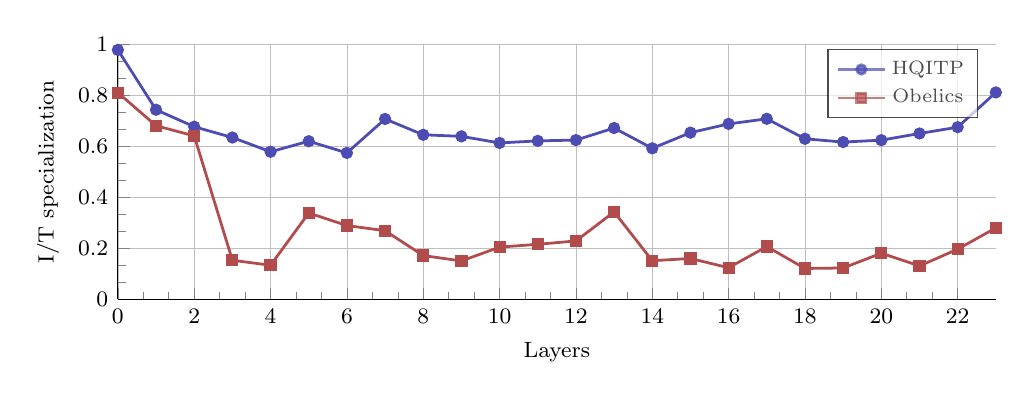
\begin{tikzpicture}
\begin{axis}[
    grid=major, %
    grid style={line width=.1pt, draw=gray!30}, %
    major grid style={line width=.2pt,draw=gray!50},
    minor tick num=2,
    axis x line*=bottom,
    axis y line*=left,
    xmin=0,
    xmax=23,
    ymin=0.0,
    ymax=1.0,
    height=1.9in,
    width=1.05\linewidth,
    ylabel style={align=center, font=\footnotesize},
    xlabel style={font=\footnotesize},
    ylabel=\footnotesize{I/T specialization},
    xlabel={\footnotesize{Layers}},
    ytick distance=0.2,
    yticklabel style={font=\footnotesize, /pgf/number format/fixed, /pgf/number format/precision=2},
    xticklabel style={font=\footnotesize},
    xtick={0,2,4,6,8,10,12,14,16,18,20,22},
    xticklabels={0,2,4,6,8,10,12,14,16,18,20,22},
    mark options={solid},
    legend style={cells={align=left}, font=\scriptsize, text=black, opacity=0.7}, %
]

\addplot[color=blue!40!gray, mark=*, mark size=1.7pt, line width=1pt] plot coordinates {  %
(0, 0.9769479348349329)
(1, 0.7427025603097698)
(2, 0.6762374582380828)
(3, 0.6340138224507533)
(4, 0.5783047019889138)
(5, 0.6195673358863271)
(6, 0.5737861572855565)
(7, 0.7066104505575633)
(8, 0.6446960774170309)
(9, 0.6386074080824291)
(10, 0.6128197724774395)
(11, 0.620867456928868)
(12, 0.6240480502092688)
(13, 0.6712385178771478)
(14, 0.591805441066985)
(15, 0.6531511085896324)
(16, 0.6873617200378165)
(17, 0.7072043647262733)
(18, 0.6290614078343542)
(19, 0.6162376387022552)
(20, 0.6237776803436119)
(21, 0.649774290665718)
(22, 0.6745086003424091)
(23, 0.810597818982423)
};
\addlegendentry{HQITP}

\addplot[color=red!40!gray, mark=square*, mark size=1.7pt, line width=1pt] plot coordinates { %
(0, 0.8098464848229123)
(1, 0.6803114998878562)
(2, 0.640428138604904)
(3, 0.15356616480436047)
(4, 0.13402442087930844)
(5, 0.33860156581505885)
(6, 0.2894806232076399)
(7, 0.269278406260023)
(8, 0.17195894943324286)
(9, 0.15091557473173656)
(10, 0.2050356661788283)
(11, 0.21603190628094793)
(12, 0.22923064654990588)
(13, 0.34291773221125066)
(14, 0.15175535984919586)
(15, 0.16059145647036643)
(16, 0.12438172525723101)
(17, 0.20722842981400202)
(18, 0.12145399323126793)
(19, 0.12335098001817868)
(20, 0.1811717532056517)
(21, 0.13129565163316004)
(22, 0.19701360887683683)
(23, 0.28035775702112686)
};
\addlegendentry{Obelics}
\end{axis}


\end{tikzpicture}

\caption{\textbf{MoE specialization.} Entropy-based image/text specialization (see~\cref{sec:specialization}) across layers for two data sources: HQITP and Obelics. 
\edit{Both sources exhibit a similar trend: the score decreases in the early layers
before increasing again in the final layers.}}
\label{fig:tokens_specialization}

    \end{minipage}
    \vspace{3mm}
\end{figure}


\section{Related Work}
\label{sec:related_work}

In this section, we review areas mostly related to our work, \ie, image retrieval and visual place recognition.

\subsection{Image Retrieval}

Image retrieval is a fundamental and well-established task in computer vision that involves searching for images similar to a given query within a large database.
The process of image retrieval typically consists of two stages: global retrieval and re-ranking. In the first stage, a global descriptor that aggregates local features is used to retrieve $k$ candidates from a large database. This is followed by spatial verification through local feature matching to re-rank these $k$ candidates. Early research relied on handcrafted features \cite{Lowe2004DistinctiveIF, BAY2008346}, while current methods utilize deep networks to learn informative representations \cite{cao2020unifyingdeeplocalglobal, radenović2018finetuningcnnimageretrieval}.

Most image retrieval methods focus on selecting diverse relevant images to help users discover options that align with their interests or needs in real-world applications \cite{Wan2014DeepLF}. Although these methods are effective in retrieving similar images, they often lack the emphasis on distinguishing between categories or achieving precise ReID \cite{10.1145/1348246.1348248}.
In \mbox{contrast}, our approach prioritizes achieving accurate ReID. Following a ``global retrieval and re-ranking" pipeline, we first use global context features to identify the top five room candidates. Our object-aware mechanism then refines the search in a coarse-to-fine manner, progressively distinguishing among candidates until the most similar room is \mbox{identified}, yielding accurate results.

\begin{figure*}[ht]
    \centering
    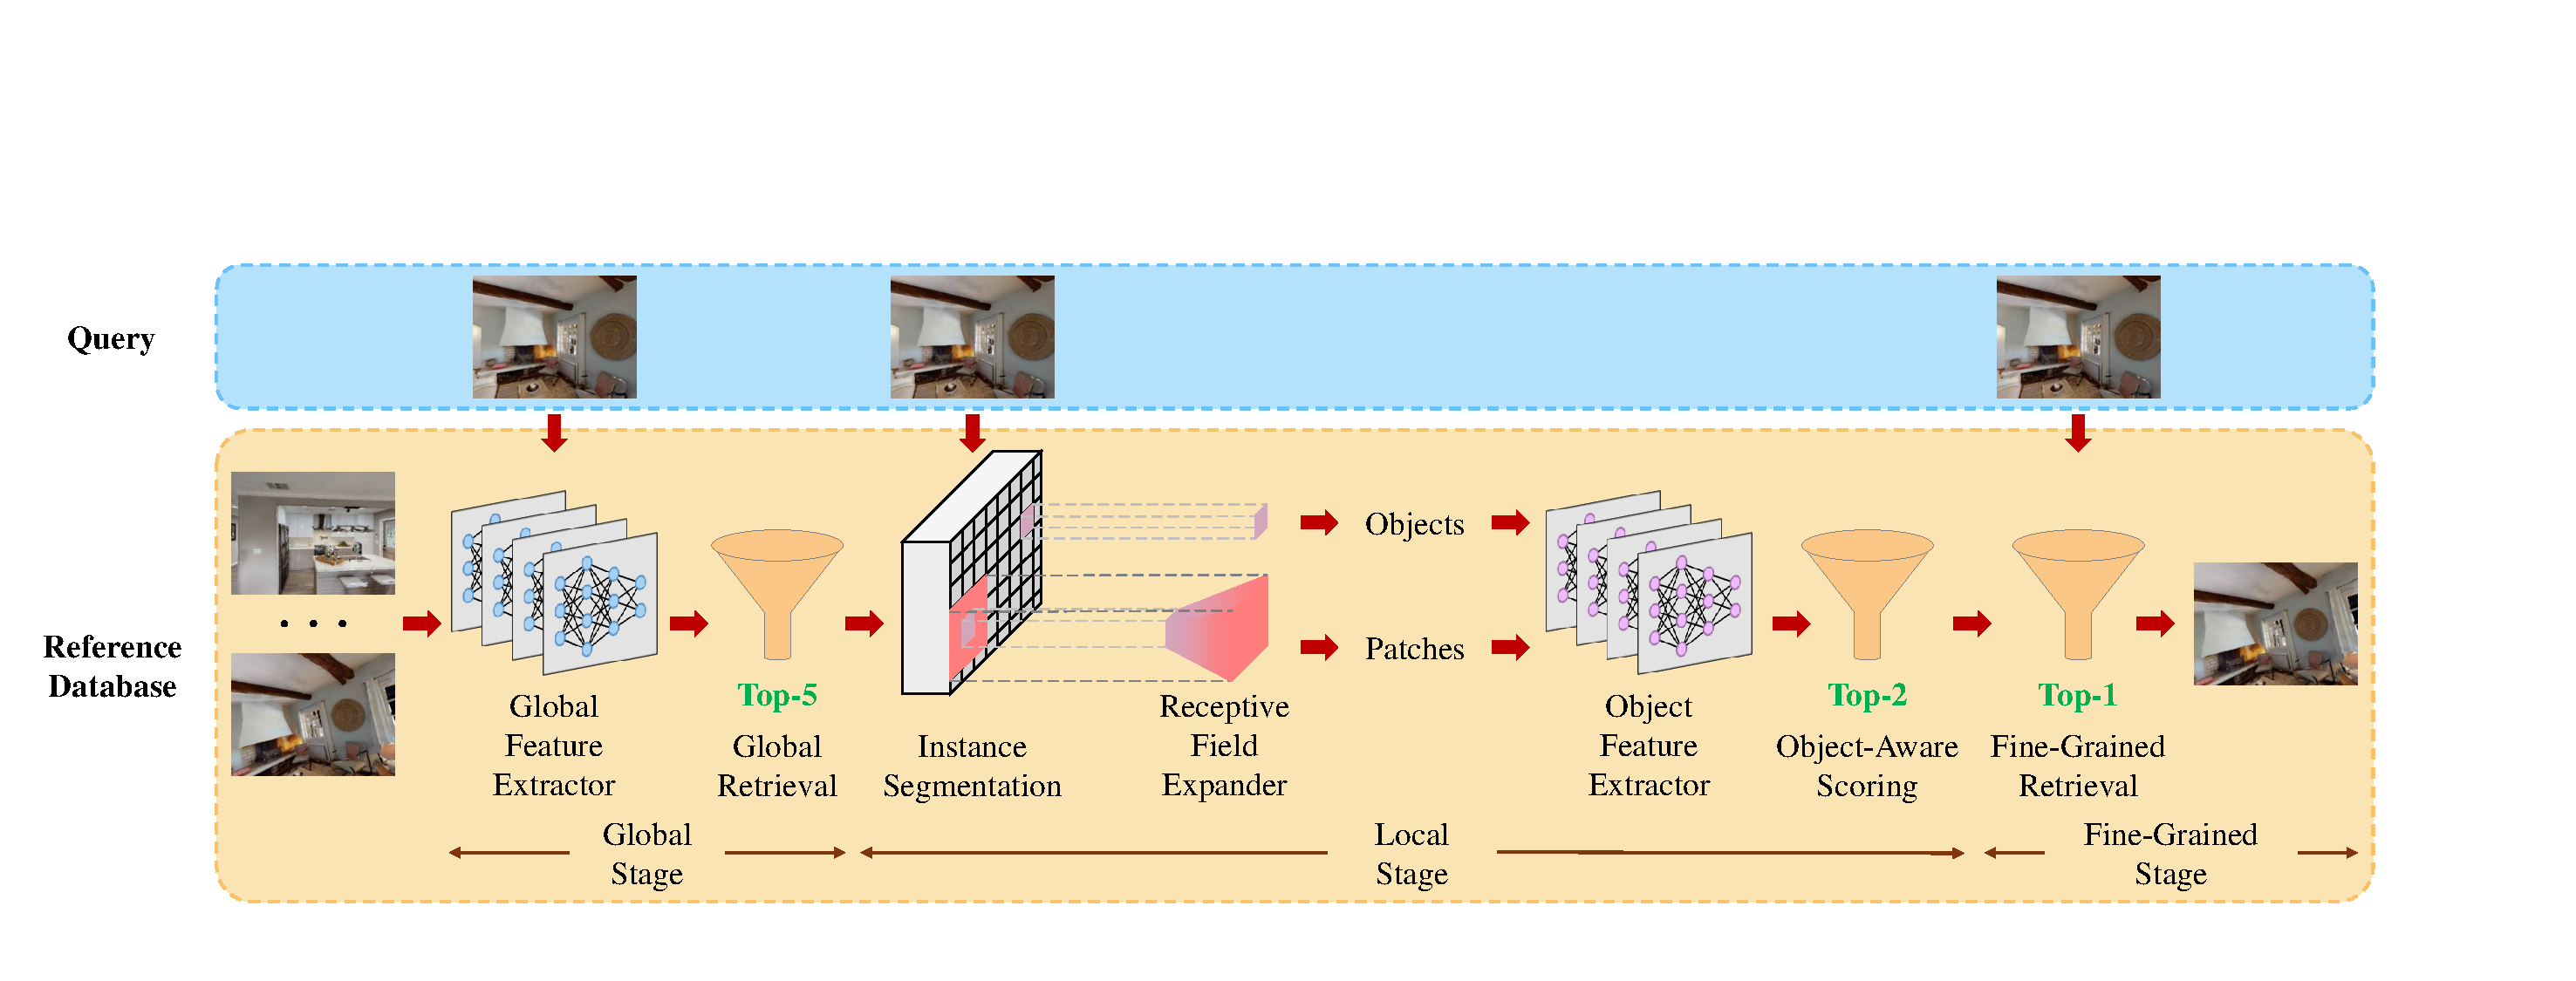
\includegraphics[width=\textwidth]{pipeline_font.pdf}
    \vspace{-16pt}
    \caption{\textbf{The AirRoom coarse-to-fine pipeline}. The pipeline begins with the Global Feature Extractor, which captures global context features to retrieve the top-5 reference images. Instance segmentation then generates object masks, followed by the Receptive Field Expander, which extracts object patches. The Object Feature Extractor processes both object and patch features. The Object-Aware Scoring module narrows the selection to the top-2 candidates, and Fine-Grained Retrieval identifies the most suitable reference image.}
    \vspace{-15pt}
    \label{fig:pipeline}
\end{figure*}

\subsection{Visual Place Recognition}

Visual place recognition (VPR) is often framed as a special image retrieval problem, aiming to match a view of a location with an image of the same place taken under different conditions.
Previous methods fall into two categories: those that directly use global descriptors and those that aggregate local features into a global descriptor. Earlier approaches that relied on global descriptors primarily used CNN-based backbones, such as ResNet \cite{he2015deepresiduallearningimage}, to generate these descriptors. More recent methods, however, leverage foundation models like DINOv2 \cite{oquab2024dinov2learningrobustvisual} for enhanced feature representation. In the aggregation category, early techniques employed handcrafted features like SIFT \cite{Lowe2004DistinctiveIF}, SURF \cite{10.1007/11744023_32}, and ORB \cite{6126544}. Later advancements, including the NetVLAD series \cite{arandjelović2016netvladcnnarchitectureweakly, hausler2021patchnetvladmultiscalefusionlocallyglobal} and AnyLoc \cite{keetha2023anylocuniversalvisualplace}, adopted learning-based models to extract feature maps and combine local features into comprehensive global descriptors.

However, the high performance of most VPR approaches is largely attributed to large-scale training on VPR-specific datasets \cite{keetha2023anylocuniversalvisualplace}. Collecting extensive data for outdoor scenes is relatively straightforward due to natural variations in daylight, weather, and seasons. However, such data collection is more challenging in indoor rooms, making large-scale training on indoor datasets difficult and potentially limiting their effectiveness.
Our approach effectively tackles this challenge by focusing on object-oriented feature representations, allowing us to leverage mature, pre-trained models for object feature learning. This design enables AirRoom to deliver robust performance without requiring any additional training or fine-tuning on specific datasets.
% Our approach addresses this challenge by centering on objects within indoor spaces, leveraging object-related feature representations. Additionally, AirRoom benefits from mature, pre-trained models for object-centric feature learning. This design enables our approach to deliver robust performance without the need for additional training or fine-tuning on specific datasets.


\section{\edit{Discussion and }Limitations} 

\cpar{\edit{Scaling laws for multimodal data mixtures.}} Our scaling laws study
spans different model configurations and training mixtures. While results
suggest that the scaling law coefficients remain largely consistent across
mixtures, a broader exploration of mixture variations is needed to validate this
observation and establish a unified scaling law that accounts for this factor.  

\cpar{\edit{Scaling laws and performance on downstream tasks.}} Similar to
previous scaling law studies, our analysis focuses on pretraining performance as
measured by the validation loss. However, the extent to which these findings
translate to downstream performance remains an open question and requires
further investigation.

\cpar{\edit{Extrapolation to larger scales.}} The accuracy of scaling law
predictions improves with increasing FLOPs~\cref{app:scaling_laws}.
\edit{Furthermore, we validate our laws when extrapolating to larger model sizes
(\cref{sec:scaling_laws_evaluation}).} However, whether these laws can be reliably
extrapolated to extremely large model sizes remains an open question. 

\cpar{\edit{High resolution and early-fusion models.}} Training early-fusion
models with high-resolution inputs leads to a significant increase in vision
tokens. While pooling techniques have been widely adopted for late-fusion
models, alternative approaches may be necessary for early fusion. \edit{Given
the similarity of early-fusion models to LLMs, it appears that techniques for
extending context length could be beneficial.}

\cpar{\edit{Scaling laws for multimodal MoEs models.}} For MoEs, we consider
only a single configuration (top-1 routing with 8 experts). \edit{We found this
configuration to work reasonably well in our setup, and follow a standard MoEs
implementation}. However, the findings may vary when optimizing \edit{more} the
MoE architecture or exploring different load-balancing, routing strategies
\edit{or different experts implementations}.

\section{Conclusion} 
We explore various strategies for compute-optimal pretraining of native
multimodal models. We found the NMMs follow similar scaling laws to those of
LLMs. Contrary to common belief, we find no inherent advantage in adopting
late-fusion architectures over early-fusion ones. While both architectures
exhibit similar scaling properties, early-fusion models are more efficient to
train and outperform late-fusion models at lower compute budgets. Furthermore,
we show that sparse architectures encourage modality-specific specialization,
leading to performance improvements while maintaining the same inference cost.




\section*{\edit{Acknowledgment}} We thank Philipp Dufter, Samira Abnar, Xiujun
Li, Zhe Gan, Alexander Toshev, Yinfei Yang, Dan Busbridge, and Jason Ramapuram
for many fruitful discussions. We thank Denise Hui, and Samy Bengio for infra
and compute support. Finally, we thank, Louis Béthune, Pierre Ablin, Marco
Cuturi, and the MLR team at Apple for their support throughout the project.
{
    \small
    \bibliographystyle{ieeenat_fullname}
    \bibliography{main}
}
\clearpage
\appendix
\addcontentsline{toc}{section}{Appendix} %
\renewcommand\ptctitle{Appendices}
\part{}
\parttoc
\clearpage
\clearpage
\appendix
\setcounter{page}{1}
\maketitlesupplementary

\section{Implementation Details}
We follow prior studies\cite{coop, cocoop, prograd, kgcoop, maple, tcp, mma} and adopt a 16-shot learning setting across all experiments, except for the few-shot learning tasks. The ViT-B/16\cite{vit} variant of the CLIP model serves as the visual backbone for all experimental setups. Hand-crafted text prompts from prior methods\cite{clip, coop, tip-adapter} are utilized and described in detail in \cref{datasets}. Optimization is performed using the AdamW optimizer with an initial learning rate of 0.001. All our models are trained with mix-precision for speeding up. For the larger ImageNet dataset, we employ a batch size of 32, while a batch size of 4 is used for all other datasets. Training on ImageNet for the base-to-novel generalization task spans 5 epochs, whereas training on the remaining datasets is conducted over 10 epochs. For cross-dataset evaluation and domain generalization tasks, we perform training for a single epoch on ImageNet. In the few-shot learning tasks, training is carried out for 5 epochs on ImageNet and 50 epochs for other datasets. The average accuracy is reported over three independent runs, with all experiments executed on a single NVIDIA RTX 4090 GPU.

Representation tokens are initialized from a zero-mean Gaussian distribution with a standard deviation of 0.02. We set $J = 6$, integrating the representation tokens beginning at the 6-th transformer layer. The dimension of the representation space, $d_r$, is set to 2048 for EuroSAT and 512 for all other datasets. Note that since the $d_r$ setting for EuroSAT differs from other datasets, in the $d_r$ ablation experiments we fix $d_r$ for EuroSAT to 2048 while adjusting $d_r$ on the other datasets. The number of representation tokens, $K$, is configured to 5. The parameter $\alpha$ is fixed at 0.7, and the details regarding the configuration of $\lambda$ are provided in \cref{ablation_lambda}.



\section{Dataset Details}
Details of 14 datasets are shown in \cref{datasets}.


\section{Computational Cost}
Table \ref{computational_cost} summarizes the learnable parameters, training time per image, total training duration, inference speed (measured in frames per second, FPS, with a batch size of 100), and the final HM metric for each approach. Our proposed model, MMRL, demonstrates a compelling balance of computational efficiency and performance. The key observations are as follows:
\begin{itemize}
    \item Models incorporating multimodal interaction mechanisms (e.g., MaPLe, MMA, and MMRL) generally involve a higher parameter count compared to models without such mechanisms.
    \item Both MMRL and the prior MMA approach exhibit significantly faster training speed, thereby reducing overall computational costs. While MaPLe and PromptSRC achieve higher inference speeds, their training durations are relatively longer. Notably, MMRL offers faster inference compared to MMA and MetaPrompt.
    \item To assess the performance of MMRL under constrained computational resources, we reduced the dimensionality of the representation space from 512 to 32. In this configuration, MMRL achieves a parameter count comparable to that of MMA, while still significantly outperforming the previous state-of-the-art model.
\end{itemize}



\begin{table}[h]
\centering
\renewcommand\arraystretch{1.25}
\caption{All methods were trained on a single NVIDIA RTX 4090 GPU using the ImageNet dataset. Each model was implemented with publicly available code and default configurations as described in their respective papers \cite{maple, promptsrc, provp, metaprompt, tcp, mma}. `V-L' denotes vision-language interaction, indicating that efficient fine-tuning incorporates interactions between visual and textual modalities before prediction. `V, L' signifies separate fine-tuning of each modality without inter-modal interaction before prediction, while `L' refers to fine-tuning limited to the textual modality alone. `Train time' is reported as both time per image and the total duration for training the full dataset(16-shots), while `FPS (100 BS)' indicates frames per second with a batch size of 100 during inference.}
\label{computational_cost}
\resizebox{0.475\textwidth}{!}{
    \begin{tabular}{@{}l|ccccc|c@{}}
    \toprule
    \multirow{2}{*}{Method} & \multirow{2}{*}{Modality} & Params & Train time & Train time & FPS & \multirow{2}{*}{HM} \\
               &     & (learnable) & (ms/image) & (minute/all) & (100 BS) &       \\ \midrule
    MaPLe      & V-L & 3.555M      & 39.5       & 26.4         & 1757.6   & 78.55 \\
    PromptSRC  & V,L & 0.046M      & 40.0       & 106.8        & 1764.2   & 79.97 \\
    ProVP      & V   & 0.147M      & 4.4        & 107.2        & 928.9    & 78.76 \\
    MetaPrompt & V,L & 0.031M      & 30.7       & 32.8         & 659.8    & 79.09 \\
    TCP        & L   & 0.332M      & 5.3        & 17.7         & 950.6    & 79.51 \\
    MMA        & V-L & 0.675M      & 2.2        & 1.5          & 688.5    & 79.87 \\ \midrule
    MMRL       & V-L & 4.992M      & 5.3        & 3.6          & 762.4    & 81.20 \\
    MMRL*      & V-L & 0.689M      & 5.3        & 3.6          & 767.8    & 80.84 \\ \bottomrule
    \end{tabular}
}
\end{table}


\section{Ablation Analysis on $\lambda$}
As shown in \cref{ablation_lambda}, increasing the value of $\lambda$ generally improves performance, with the optimal or near-optimal results typically observed when $\lambda$ is set between 4 and 6 across most datasets. Notably, as $\lambda$ continues to increase, its impact on model performance within the same dataset diminishes, indicating reduced sensitivity to variations in $\lambda$. This trend suggests that the model becomes more robust and less reliant on precise tuning of $\lambda$ at higher values.


\begin{table*}[h]
\centering
\caption{Summary of the 14 datasets.}
\label{datasets}
\renewcommand\arraystretch{1.2}
\resizebox{1.0\textwidth}{!}{
    \begin{tabular}{@{}l|llllll@{}}
    \toprule
    Dataset      & Classes & Train  & Val    & Test   & Description                         & Prompt                                \\ \midrule
    ImageNet     & 1000    & 1.28M  & $\sim$ & 50000  & Recognition of generic objects      & ``a photo of a [CLASS].”              \\
    Caltech101   & 100     & 4128   & 1649   & 2465   & Recognition of generic objects      & ``a photo of a [CLASS].”              \\
    OxfordPets      & 37    & 2944   & 736    & 3669   & Fine-grained classification of pets                    & ``a photo of a [CLASS], a type of pet.”      \\
    StanfordCars & 196     & 6509   & 1635   & 8041   & Fine-grained classification of cars & ``a photo of a [CLASS].”              \\
    Flowers102      & 102   & 4093   & 1633   & 2463   & Fine-grained classification of flowers                 & ``a photo of a [CLASS], a type of flower.”   \\
    Food101         & 101   & 50500  & 20200  & 30300  & Fine-grained classification of foods                   & ``a photo of [CLASS], a type of food.”       \\
    FGVCAircraft    & 100   & 3334   & 3333   & 3333   & Fine-grained classification of aircrafts               & ``a photo of a [CLASS], a type of aircraft.” \\
    SUN397       & 397     & 15880  & 3970   & 19850  & Scene classification                & ``a photo of a [CLASS].”              \\
    DTD          & 47      & 2820   & 1128   & 1692   & Texture classification              & ``[CLASS] texture.”                   \\
    EuroSAT         & 10    & 13500  & 5400   & 8100   & Land use \& cover classification with satellite images & ``a centered satellite photo of [CLASS].”    \\
    UCF101       & 101     & 7639   & 1898   & 3783   & Action recognition                  & ``a photo of a person doing [CLASS].” \\ \midrule
    ImageNetV2   & 1,000   & $\sim$ & $\sim$ & 10,000 & New test data for ImageNet          & ``a photo of a [CLASS].”              \\
    ImageNet-Sketch & 1,000 & $\sim$ & $\sim$ & 50,889 & Sketch-style images of ImageNet classes                & ``a photo of a [CLASS].”                     \\
    ImageNet-A      & 200   & $\sim$ & $\sim$ & 7,500  & Natural adversarial examples of 200 ImageNet classes   & ``a photo of a [CLASS].”                     \\
    ImageNet-R   & 200     & $\sim$ & $\sim$ & 30,000 & Renditions of 200 ImageNet classes  & ``a photo of a [CLASS].”              \\ \bottomrule
    \end{tabular}
    }
\end{table*}


\begin{table*}[h]
\centering
\caption{Ablation on $\lambda$ across 11 datasets, with results evaluated using the harmonic mean (HM) metric.}
\label{ablation_lambda}
\renewcommand\arraystretch{1.2}
\resizebox{1.0\textwidth}{!}{
    \begin{tabular}{@{}c|ccccccccccc@{}}
    \toprule
    $\alpha$ & ImageNet       & Caltech101     & OxfordPets & StanfordCars & Flowers102 & Food101 & FGVCAircraft   & SUN397         & DTD            & EuroSAT & UCF101 \\ \midrule
    0.0  & 74.01 & 95.97 & 96.35          & 76.00          & 84.42          & 90.10          & 38.52 & 79.67 & 68.21 & 82.65          & 81.63          \\
    0.01 & 74.07 & 96.12 & 96.39          & 75.95          & 84.82          & 90.23          & 37.87 & 79.85 & 67.73 & \textbf{87.21} & 82.11          \\
    0.1  & 74.23 & 96.25 & 96.49          & 76.32          & 84.81          & 90.53          & 38.66 & 80.23 & 69.79 & 83.21          & 82.91          \\
    0.2  & 74.38 & 96.40 & \textbf{96.74} & 76.67          & 85.31          & 90.61          & 39.27 & 80.25 & 70.58 & 82.68          & 82.70          \\
    0.5      & \textbf{74.45} & \textbf{96.68} & 96.54      & 77.09        & 85.74      & 90.86   & 40.37          & 80.61          & 72.67          & 82.87   & 83.05  \\
    3.0  & 74.09 & 96.59 & 96.51          & 77.72          & 86.65          & 90.98          & 40.48 & 81.10 & 73.54 & 77.95          & \textbf{83.89} \\
    4.0  & 74.04 & 96.62 & 96.55          & 77.73          & \textbf{86.78} & 90.98          & 40.66 & 81.14 & 73.75 & 77.27          & 83.45          \\
    5.0  & 73.93 & 96.62 & 96.60          & 77.86          & 86.42          & \textbf{91.03} & 40.42 & 81.07 & 73.69 & 78.05          & 83.84          \\
    6.0      & 73.83          & 96.61          & 96.66      & 78.05        & 86.48      & 91.00   & \textbf{41.15} & \textbf{81.20} & \textbf{73.82} & 75.23   & 83.68  \\
    7.0  & 73.78 & 96.62 & 96.58          & \textbf{78.06} & 86.53          & 90.95          & 40.88 & 81.10 & 73.65 & 75.85          & 83.55          \\
    10.0 & 73.68 & 96.64 & 96.56          & 77.86          & 86.46          & 91.00          & 41.01 & 80.93 & 73.68 & 77.61          & 83.38          \\ \bottomrule
    \end{tabular}
}
\end{table*}

\begin{table}[t]
\small
\centering
\caption{Ablation on different regularization strategies.}
\label{ablation_regularization}
\begin{tabular}{@{}c|ccc@{}}
\toprule
Regularization & Base           & Novel          & HM             \\ \midrule
\rowcolor[HTML]{EFEFEF} 
Cosine         & \textbf{85.68} & \textbf{77.16} & \textbf{81.20} \\
L1             & 85.46          & 76.03          & 80.47          \\
MSE             & 85.13          & 74.62          & 79.53          \\ \bottomrule
\end{tabular}
\end{table}

\section{Ablation Analysis on Regularization Strategies}
We investigate the impact of various regularization strategies aimed at maximizing the similarity between class token features and frozen CLIP features to retain pre-trained knowledge. The results, summarized in \cref{ablation_regularization}, indicate that cosine regularization achieves the best performance. In contrast, both L1 and MSE losses lead to performance degradation, with MSE causing a significant decline. This result can be attributed to the more relaxed and flexible constraints of cosine regularization, enabling the class token to preserve generalizability while effectively capturing task-specific knowledge.






\section{Few-Shot Learning}
\cref{few_shot1,few_shot2} provide detailed comparisons of MMRL and prior state-of-the-art methods on few-shot learning across 11 datasets. MMRL achieves the highest average performance across all shots. Note that the MMA results are reproduced from the open-source code, as the original paper does not report results for this experiment.







\begin{table*}[t]
\small
\centering
\caption{Comparison of MMRL with previous state-of-the-art methods on few-shot learning across 11 datasets.}
\label{few_shot1}
\setlength{\tabcolsep}{15pt}{
\resizebox{0.9\textwidth}{!}{
    \begin{tabular}{@{}ll|ccccc}
    \toprule
    \textbf{Dataset} &
      \textbf{Method} &
      \textbf{1 shot} &
      \textbf{2 shots} &
      \textbf{4 shots} &
      \textbf{8 shots} &
      \textbf{16 shots} \\ \midrule
     &
      Linear probe CLIP &
      45.83 &
      57.98 &
      68.01 &
      74.47 &
      78.79 \\
     &
      CoOp &
      67.56 &
      70.65 &
      74.02 &
      76.98 &
      79.89 \\
     &
      CoCoOp &
      66.79 &
      67.65 &
      71.21 &
      72.96 &
      74.90 \\
     &
      MaPLe &
      69.27 &
      72.58 &
      75.37 &
      78.89 &
      81.79 \\
     &
      PromptSRC &
      72.32 &
      75.29 &
      78.35 &
      80.69 &
      82.87 \\
     &
      MMA &
      69.28 &
      72.08 &
      76.38 &
      79.57 &
      82.76 \\
    \multirow{-7}{*}{Average} &
      \cellcolor[HTML]{E8E8E8}$\text{MMRL}_{\text{ (Ours)}}$ &
      \cellcolor[HTML]{E8E8E8}\textbf{72.67} &
      \cellcolor[HTML]{E8E8E8}\textbf{75.90} &
      \cellcolor[HTML]{E8E8E8}\textbf{79.20} &
      \cellcolor[HTML]{E8E8E8}\textbf{81.47} &
      \cellcolor[HTML]{E8E8E8}\textbf{84.34} \\ \midrule
     &
      Linear probe CLIP &
      32.13 &
      44.88 &
      54.85 &
      62.23 &
      67.31 \\
     &
      CoOp &
      66.33 &
      67.07 &
      68.73 &
      70.63 &
      71.87 \\
     &
      CoCoOp &
      69.43 &
      69.78 &
      70.39 &
      70.63 &
      70.83 \\
     &
      MaPLe &
      62.67 &
      65.10 &
      67.70 &
      70.30 &
      72.33 \\
     &
      PromptSRC &
      68.13 &
      69.77 &
      71.07 &
      \textbf{72.33} &
      73.17 \\
     &
      MMA &
      \textbf{69.17} &
      \textbf{70.37} &
      71.00 &
      71.77 &
      73.13 \\
    \multirow{-7}{*}{ImageNet} &
      \cellcolor[HTML]{E8E8E8}$\text{MMRL}_{\text{ (Ours)}}$ &
      \cellcolor[HTML]{E8E8E8}69.00 &
      \cellcolor[HTML]{E8E8E8}70.30 &
      \cellcolor[HTML]{E8E8E8}\textbf{71.40} &
      \cellcolor[HTML]{E8E8E8}\textbf{72.33} &
      \cellcolor[HTML]{E8E8E8}\textbf{73.40} \\ \midrule
     &
      Linear probe CLIP &
      79.88 &
      89.01 &
      92.05 &
      93.41 &
      95.43 \\
     &
      CoOp &
      92.60 &
      93.07 &
      94.40 &
      94.37 &
      95.57 \\
     &
      CoCoOp &
      93.83 &
      94.82 &
      94.98 &
      95.04 &
      95.16 \\
     &
      MaPLe &
      92.57 &
      93.97 &
      94.43 &
      95.20 &
      96.00 \\
     &
      PromptSRC &
      93.67 &
      94.53 &
      95.27 &
      95.67 &
      96.07 \\
     &
      MMA &
      92.90 &
      94.00 &
      94.33 &
      95.37 &
      96.33 \\
    \multirow{-7}{*}{Caltech101} &
      \cellcolor[HTML]{E8E8E8}$\text{MMRL}_{\text{ (Ours)}}$ &
      \cellcolor[HTML]{E8E8E8}\textbf{94.17} &
      \cellcolor[HTML]{E8E8E8}\textbf{94.83} &
      \cellcolor[HTML]{E8E8E8}\textbf{96.03} &
      \cellcolor[HTML]{E8E8E8}\textbf{96.27} &
      \cellcolor[HTML]{E8E8E8}\textbf{97.13} \\ \midrule
     &
      Linear probe CLIP &
      44.06 &
      58.37 &
      71.17 &
      78.36 &
      85.34 \\
     &
      CoOp &
      90.37 &
      89.80 &
      92.57 &
      91.27 &
      91.87 \\
     &
      CoCoOp &
      91.27 &
      \textbf{92.64} &
      92.81 &
      93.45 &
      93.34 \\
     &
      MaPLe &
      89.10 &
      90.87 &
      91.90 &
      92.57 &
      92.83 \\
     &
      PromptSRC &
      \textbf{92.00} &
      92.50 &
      \textbf{93.43} &
      \textbf{93.50} &
      93.67 \\
     &
      MMA &
      91.23 &
      91.97 &
      92.23 &
      92.77 &
      93.23 \\
    \multirow{-7}{*}{OxfordPets} &
      \cellcolor[HTML]{E8E8E8}$\text{MMRL}_{\text{ (Ours)}}$ &
      \cellcolor[HTML]{E8E8E8}90.87 &
      \cellcolor[HTML]{E8E8E8}91.57 &
      \cellcolor[HTML]{E8E8E8}92.57 &
      \cellcolor[HTML]{E8E8E8}93.03 &
      \cellcolor[HTML]{E8E8E8}\textbf{93.83} \\ \midrule
     &
      Linear probe CLIP &
      35.66 &
      50.28 &
      63.38 &
      73.67 &
      80.44 \\
     &
      CoOp &
      67.43 &
      70.50 &
      74.47 &
      79.30 &
      83.07 \\
     &
      CoCoOp &
      67.22 &
      68.37 &
      69.39 &
      70.44 &
      71.57 \\
     &
      MaPLe &
      66.60 &
      71.60 &
      75.30 &
      79.47 &
      83.57 \\
     &
      PromptSRC &
      \textbf{69.40} &
      \textbf{73.40} &
      77.13 &
      80.97 &
      83.83 \\
     &
      MMA &
      67.87 &
      71.77 &
      76.50 &
      81.40 &
      85.70 \\
    \multirow{-7}{*}{StanfordCars} &
      \cellcolor[HTML]{E8E8E8}$\text{MMRL}_{\text{ (Ours)}}$ &
      \cellcolor[HTML]{E8E8E8}68.70 &
      \cellcolor[HTML]{E8E8E8}72.93 &
      \cellcolor[HTML]{E8E8E8}\textbf{78.17} &
      \cellcolor[HTML]{E8E8E8}\textbf{82.57} &
      \cellcolor[HTML]{E8E8E8}\textbf{86.43} \\ \midrule
     &
      Linear probe CLIP &
      69.74 &
      85.07 &
      92.02 &
      96.10 &
      97.37 \\
     &
      CoOp &
      77.53 &
      87.33 &
      92.17 &
      94.97 &
      97.07 \\
     &
      CoCoOp &
      72.08 &
      75.79 &
      78.40 &
      84.30 &
      87.84 \\
     &
      MaPLe &
      83.30 &
      88.93 &
      92.67 &
      95.80 &
      97.00 \\
     &
      PromptSRC &
      85.93 &
      91.17 &
      93.87 &
      96.27 &
      97.60 \\
     &
      MMA &
      83.60 &
      90.30 &
      93.00 &
      95.97 &
      97.97 \\
    \multirow{-7}{*}{Flowers102} &
      \cellcolor[HTML]{E8E8E8}$\text{MMRL}_{\text{ (Ours)}}$ &
      \cellcolor[HTML]{E8E8E8}\textbf{85.97} &
      \cellcolor[HTML]{E8E8E8}\textbf{91.20} &
      \cellcolor[HTML]{E8E8E8}\textbf{94.60} &
      \cellcolor[HTML]{E8E8E8}\textbf{96.60} &
      \cellcolor[HTML]{E8E8E8}\textbf{98.40} \\ \bottomrule
    \end{tabular}
    }
    }
\end{table*}


\begin{table*}[t]
\small
\centering
\caption{Comparison of MMRL with previous state-of-the-art methods on few-shot learning across 11 datasets.}
\label{few_shot2}
\setlength{\tabcolsep}{15pt}{
\resizebox{0.9\textwidth}{!}{
    \begin{tabular}{@{}ll|ccccc}
    \toprule
    \textbf{Dataset} &
      \textbf{Method} &
      \textbf{1 shot} &
      \textbf{2 shots} &
      \textbf{4 shots} &
      \textbf{8 shots} &
      \textbf{16 shots} \\ \midrule
     &
      Linear probe CLIP &
      43.96 &
      61.51 &
      73.19 &
      79.79 &
      82.90 \\
     &
      CoOp &
      84.33 &
      84.40 &
      84.47 &
      82.67 &
      84.20 \\
     &
      CoCoOp &
      \textbf{85.65} &
      \textbf{86.22} &
      \textbf{86.88} &
      \textbf{86.97} &
      87.25 \\
     &
      MaPLe &
      80.50 &
      81.47 &
      81.77 &
      83.60 &
      85.33 \\
     &
      PromptSRC &
      84.87 &
      85.70 &
      86.17 &
      86.90 &
      \textbf{87.50} \\
     &
      MMA &
      83.03 &
      82.50 &
      82.13 &
      83.00 &
      84.57 \\
    \multirow{-7}{*}{Food101} &
      \cellcolor[HTML]{E8E8E8}$\text{MMRL}_{\text{ (Ours)}}$ &
      \cellcolor[HTML]{E8E8E8}84.87 &
      \cellcolor[HTML]{E8E8E8}85.53 &
      \cellcolor[HTML]{E8E8E8}85.77 &
      \cellcolor[HTML]{E8E8E8}86.33 &
      \cellcolor[HTML]{E8E8E8}87.03 \\ \midrule
     &
      Linear probe CLIP &
      19.61 &
      26.41 &
      32.33 &
      39.35 &
      45.36 \\
     &
      CoOp &
      21.37 &
      26.20 &
      30.83 &
      39.00 &
      43.40 \\
     &
      CoCoOp &
      12.68 &
      15.06 &
      24.79 &
      26.61 &
      31.21 \\
     &
      MaPLe &
      26.73 &
      30.90 &
      34.87 &
      42.00 &
      48.40 \\
     &
      PromptSRC &
      27.67 &
      31.70 &
      37.47 &
      43.27 &
      50.83 \\
     &
      MMA &
      \textbf{28.73} &
      31.90 &
      37.57 &
      44.83 &
      52.70 \\
    \multirow{-7}{*}{FGVCAircraft} &
      \cellcolor[HTML]{E8E8E8}$\text{MMRL}_{\text{ (Ours)}}$ &
      \cellcolor[HTML]{E8E8E8}28.53 &
      \cellcolor[HTML]{E8E8E8}\textbf{34.23} &
      \cellcolor[HTML]{E8E8E8}\textbf{40.47} &
      \cellcolor[HTML]{E8E8E8}\textbf{48.07} &
      \cellcolor[HTML]{E8E8E8}\textbf{57.60} \\ \midrule
     &
      Linear probe CLIP &
      41.58 &
      53.70 &
      63.00 &
      69.08 &
      73.28 \\
     &
      CoOp &
      66.77 &
      66.53 &
      69.97 &
      71.53 &
      74.67 \\
     &
      CoCoOp &
      68.33 &
      69.03 &
      70.21 &
      70.84 &
      72.15 \\
     &
      MaPLe &
      64.77 &
      67.10 &
      70.67 &
      73.23 &
      75.53 \\
     &
      PromptSRC &
      \textbf{69.67} &
      \textbf{71.60} &
      \textbf{74.00} &
      75.73 &
      77.23 \\
     &
      MMA &
      64.00 &
      67.17 &
      69.97 &
      72.30 &
      74.63 \\
    \multirow{-7}{*}{SUN397} &
      \cellcolor[HTML]{E8E8E8}$\text{MMRL}_{\text{ (Ours)}}$ &
      \cellcolor[HTML]{E8E8E8}68.90 &
      \cellcolor[HTML]{E8E8E8}71.53 &
      \cellcolor[HTML]{E8E8E8}73.93 &
      \cellcolor[HTML]{E8E8E8}\textbf{76.00} &
      \cellcolor[HTML]{E8E8E8}\textbf{77.70} \\ \midrule
     &
      Linear probe CLIP &
      34.59 &
      40.76 &
      55.71 &
      63.46 &
      69.96 \\
     &
      CoOp &
      50.23 &
      53.60 &
      58.70 &
      64.77 &
      69.87 \\
     &
      CoCoOp &
      48.54 &
      52.17 &
      55.04 &
      58.89 &
      63.04 \\
     &
      MaPLe &
      52.13 &
      55.50 &
      61.00 &
      66.50 &
      71.33 \\
     &
      PromptSRC &
      56.23 &
      59.97 &
      65.53 &
      69.87 &
      72.73 \\
     &
      MMA &
      52.27 &
      56.90 &
      63.93 &
      67.97 &
      73.47 \\
    \multirow{-7}{*}{DTD} &
      \cellcolor[HTML]{E8E8E8}$\text{MMRL}_{\text{ (Ours)}}$ &
      \cellcolor[HTML]{E8E8E8}\textbf{56.37} &
      \cellcolor[HTML]{E8E8E8}\textbf{61.37} &
      \cellcolor[HTML]{E8E8E8}\textbf{67.87} &
      \cellcolor[HTML]{E8E8E8}\textbf{71.60} &
      \cellcolor[HTML]{E8E8E8}\textbf{75.30} \\ \midrule
     &
      Linear probe CLIP &
      49.23 &
      61.98 &
      77.09 &
      84.43 &
      87.21 \\
     &
      CoOp &
      54.93 &
      65.17 &
      70.80 &
      78.07 &
      84.93 \\
     &
      CoCoOp &
      55.33 &
      46.74 &
      65.56 &
      68.21 &
      73.32 \\
     &
      MaPLe &
      71.80 &
      78.30 &
      84.50 &
      87.73 &
      92.33 \\
     &
      PromptSRC &
      73.13 &
      79.37 &
      86.30 &
      \textbf{88.80} &
      92.43 \\
     &
      MMA &
      55.07 &
      59.80 &
      79.40 &
      86.47 &
      92.37 \\
    \multirow{-7}{*}{EuroSAT} &
      \cellcolor[HTML]{E8E8E8}$\text{MMRL}_{\text{ (Ours)}}$ &
      \cellcolor[HTML]{E8E8E8}\textbf{76.00} &
      \cellcolor[HTML]{E8E8E8}\textbf{82.87} &
      \cellcolor[HTML]{E8E8E8}\textbf{87.67} &
      \cellcolor[HTML]{E8E8E8}88.73 &
      \cellcolor[HTML]{E8E8E8}\textbf{93.37} \\ \midrule
     &
      Linear probe CLIP &
      53.66 &
      65.78 &
      73.28 &
      79.34 &
      82.11 \\
     &
      CoOp &
      71.23 &
      73.43 &
      77.10 &
      80.20 &
      82.23 \\
     &
      CoCoOp &
      70.30 &
      73.51 &
      74.82 &
      77.14 &
      78.14 \\
     &
      MaPLe &
      71.83 &
      74.60 &
      78.47 &
      81.37 &
      85.03 \\
     &
      PromptSRC &
      74.80 &
      \textbf{78.50} &
      81.57 &
      84.30 &
      86.47 \\
     &
      MMA &
      74.17 &
      76.17 &
      80.10 &
      83.43 &
      86.30 \\
    \multirow{-7}{*}{UCF101} &
      \cellcolor[HTML]{E8E8E8}$\text{MMRL}_{\text{ (Ours)}}$ &
      \cellcolor[HTML]{E8E8E8}\textbf{75.97} &
      \cellcolor[HTML]{E8E8E8}\textbf{78.50} &
      \cellcolor[HTML]{E8E8E8}\textbf{82.67} &
      \cellcolor[HTML]{E8E8E8}\textbf{84.67} &
      \cellcolor[HTML]{E8E8E8}\textbf{87.60} \\ \bottomrule
    \end{tabular}
    }
    }
\end{table*}




\end{document}
